\documentclass[twoside]{book}

% Packages required by doxygen
\usepackage{fixltx2e}
\usepackage{calc}
\usepackage{doxygen}
\usepackage[export]{adjustbox} % also loads graphicx
\usepackage{graphicx}
\usepackage[utf8]{inputenc}
\usepackage{makeidx}
\usepackage{multicol}
\usepackage{multirow}
\PassOptionsToPackage{warn}{textcomp}
\usepackage{textcomp}
\usepackage[nointegrals]{wasysym}
\usepackage[table]{xcolor}

% NLS support packages
\usepackage{hfont}

% Font selection
\usepackage[T1]{fontenc}
\usepackage[scaled=.90]{helvet}
\usepackage{courier}
\usepackage{amssymb}
\usepackage{sectsty}
\renewcommand{\familydefault}{\sfdefault}
\allsectionsfont{%
  \fontseries{bc}\selectfont%
  \color{darkgray}%
}
\renewcommand{\DoxyLabelFont}{%
  \fontseries{bc}\selectfont%
  \color{darkgray}%
}
\newcommand{\+}{\discretionary{\mbox{\scriptsize$\hookleftarrow$}}{}{}}

% Page & text layout
\usepackage{geometry}
\geometry{%
  a4paper,%
  top=2.5cm,%
  bottom=2.5cm,%
  left=2.5cm,%
  right=2.5cm%
}
\tolerance=750
\hfuzz=15pt
\hbadness=750
\setlength{\emergencystretch}{15pt}
\setlength{\parindent}{0cm}
\setlength{\parskip}{3ex plus 2ex minus 2ex}
\makeatletter
\renewcommand{\paragraph}{%
  \@startsection{paragraph}{4}{0ex}{-1.0ex}{1.0ex}{%
    \normalfont\normalsize\bfseries\SS@parafont%
  }%
}
\renewcommand{\subparagraph}{%
  \@startsection{subparagraph}{5}{0ex}{-1.0ex}{1.0ex}{%
    \normalfont\normalsize\bfseries\SS@subparafont%
  }%
}
\makeatother

% Headers & footers
\usepackage{fancyhdr}
\pagestyle{fancyplain}
\fancyhead[LE]{\fancyplain{}{\bfseries\thepage}}
\fancyhead[CE]{\fancyplain{}{}}
\fancyhead[RE]{\fancyplain{}{\bfseries\leftmark}}
\fancyhead[LO]{\fancyplain{}{\bfseries\rightmark}}
\fancyhead[CO]{\fancyplain{}{}}
\fancyhead[RO]{\fancyplain{}{\bfseries\thepage}}
\fancyfoot[LE]{\fancyplain{}{}}
\fancyfoot[CE]{\fancyplain{}{}}
\fancyfoot[RE]{\fancyplain{}{\bfseries\scriptsize 다음에 의해 생성됨 \+:  Doxygen }}
\fancyfoot[LO]{\fancyplain{}{\bfseries\scriptsize 다음에 의해 생성됨 \+:  Doxygen }}
\fancyfoot[CO]{\fancyplain{}{}}
\fancyfoot[RO]{\fancyplain{}{}}
\renewcommand{\footrulewidth}{0.4pt}
\renewcommand{\chaptermark}[1]{%
  \markboth{#1}{}%
}
\renewcommand{\sectionmark}[1]{%
  \markright{\thesection\ #1}%
}

% Indices & bibliography
\usepackage{natbib}
\usepackage[titles]{tocloft}
\setcounter{tocdepth}{3}
\setcounter{secnumdepth}{5}
\makeindex

% Hyperlinks (required, but should be loaded last)
\usepackage{ifpdf}
\ifpdf
  \usepackage[pdftex,pagebackref=true]{hyperref}
\else
  \usepackage[ps2pdf,pagebackref=true]{hyperref}
\fi
\hypersetup{%
  colorlinks=true,%
  linkcolor=blue,%
  citecolor=blue,%
  unicode%
}

% Custom commands
\newcommand{\clearemptydoublepage}{%
  \newpage{\pagestyle{empty}\cleardoublepage}%
}

\usepackage{caption}
\captionsetup{labelsep=space,justification=centering,font={bf},singlelinecheck=off,skip=4pt,position=top}

%===== C O N T E N T S =====

\begin{document}

% Titlepage & ToC
\hypersetup{pageanchor=false,
             bookmarksnumbered=true,
             pdfencoding=unicode
            }
\pagenumbering{alph}
\begin{titlepage}
\vspace*{7cm}
\begin{center}%
{\Large Secu\+Scan \\[1ex]\large 1.\+0 }\\
\vspace*{1cm}
{\large 다음에 의해 생성됨 \+:  Doxygen 1.8.13}\\
\end{center}
\end{titlepage}
\clearemptydoublepage
\pagenumbering{roman}
\tableofcontents
\clearemptydoublepage
\pagenumbering{arabic}
\hypersetup{pageanchor=true}

%--- Begin generated contents ---
\chapter{클래스 색인}
\section{클래스 목록}
다음은 클래스, 구조체, 공용체 그리고 인터페이스들입니다. (간략한 설명만을 보여줍니다) \+:\begin{DoxyCompactList}
\item\contentsline{section}{\hyperlink{struct_rule}{Rule} }{\pageref{struct_rule}}{}
\end{DoxyCompactList}

\chapter{파일 색인}
\section{파일 목록}
다음은 모든 파일에 대한 목록입니다. (간략한 설명만을 보여줍니다) \+:\begin{DoxyCompactList}
\item\contentsline{section}{bob\+\_\+secuscan/\hyperlink{decrypt__xccdf_8cpp}{decrypt\+\_\+xccdf.\+cpp} }{\pageref{decrypt__xccdf_8cpp}}{}
\item\contentsline{section}{bob\+\_\+secuscan/\hyperlink{decrypt__xccdf_8h}{decrypt\+\_\+xccdf.\+h} }{\pageref{decrypt__xccdf_8h}}{}
\item\contentsline{section}{bob\+\_\+secuscan/\hyperlink{display_8cpp}{display.\+cpp} }{\pageref{display_8cpp}}{}
\item\contentsline{section}{bob\+\_\+secuscan/\hyperlink{display_8h}{display.\+h} }{\pageref{display_8h}}{}
\item\contentsline{section}{bob\+\_\+secuscan/\hyperlink{engine_8cpp}{engine.\+cpp} }{\pageref{engine_8cpp}}{}
\item\contentsline{section}{bob\+\_\+secuscan/\hyperlink{engine_8h}{engine.\+h} }{\pageref{engine_8h}}{}
\item\contentsline{section}{bob\+\_\+secuscan/\hyperlink{html__report_8cpp}{html\+\_\+report.\+cpp} }{\pageref{html__report_8cpp}}{}
\item\contentsline{section}{bob\+\_\+secuscan/\hyperlink{html__report_8h}{html\+\_\+report.\+h} }{\pageref{html__report_8h}}{}
\item\contentsline{section}{bob\+\_\+secuscan/\hyperlink{main_8cpp}{main.\+cpp} }{\pageref{main_8cpp}}{}
\item\contentsline{section}{bob\+\_\+secuscan/\hyperlink{pdf__report_8cpp}{pdf\+\_\+report.\+cpp} }{\pageref{pdf__report_8cpp}}{}
\item\contentsline{section}{bob\+\_\+secuscan/\hyperlink{pdf__report_8h}{pdf\+\_\+report.\+h} }{\pageref{pdf__report_8h}}{}
\item\contentsline{section}{bob\+\_\+secuscan/\hyperlink{rule_8cpp}{rule.\+cpp} }{\pageref{rule_8cpp}}{}
\item\contentsline{section}{bob\+\_\+secuscan/\hyperlink{rule_8h}{rule.\+h} }{\pageref{rule_8h}}{}
\item\contentsline{section}{bob\+\_\+secuscan/\hyperlink{scoring_8cpp}{scoring.\+cpp} }{\pageref{scoring_8cpp}}{}
\item\contentsline{section}{bob\+\_\+secuscan/\hyperlink{scoring_8h}{scoring.\+h} }{\pageref{scoring_8h}}{}
\item\contentsline{section}{bob\+\_\+secuscan/\hyperlink{xml__parser_8cpp}{xml\+\_\+parser.\+cpp} }{\pageref{xml__parser_8cpp}}{}
\item\contentsline{section}{bob\+\_\+secuscan/\hyperlink{xml__parser_8h}{xml\+\_\+parser.\+h} }{\pageref{xml__parser_8h}}{}
\end{DoxyCompactList}

\chapter{클래스 문서화}
\hypertarget{struct_rule}{}\section{Rule 구조체 참조}
\label{struct_rule}\index{Rule@{Rule}}


{\ttfamily \#include $<$rule.\+h$>$}



Rule에 대한 협력 다이어그램\+:\nopagebreak
\begin{figure}[H]
\begin{center}
\leavevmode
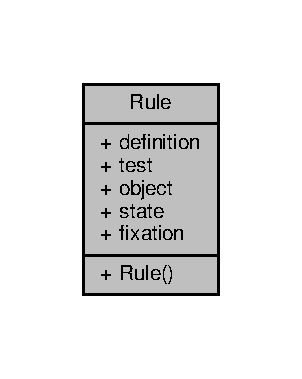
\includegraphics[width=145pt]{struct_rule__coll__graph}
\end{center}
\end{figure}
\subsection*{Public 멤버 함수}
\begin{DoxyCompactItemize}
\item 
\hyperlink{struct_rule_af2cf72df5006e2ce8c5a05666b028683}{Rule} (string def, string tst, string obj, string st, string fix)
\end{DoxyCompactItemize}
\subsection*{Public 속성}
\begin{DoxyCompactItemize}
\item 
string \hyperlink{struct_rule_a747f1497b7ed37f57b7e005bb01e1b3b}{definition}
\item 
string \hyperlink{struct_rule_a44865cab2ebf41957fd79a0ace31078b}{test}
\item 
string \hyperlink{struct_rule_aef723fe24b9b0acd063cb8cf7ba77ba1}{object}
\item 
string \hyperlink{struct_rule_a565f287f7b2370aca4f019d143227c5f}{state}
\item 
string \hyperlink{struct_rule_a580d700e40dd7c70ab0eea2a75335fb7}{fixation}
\end{DoxyCompactItemize}


\subsection{상세한 설명}
검사 룰을 표현한 클래스 

rule.\+h 파일의 6 번째 라인에서 정의되었습니다.



\subsection{생성자 \& 소멸자 문서화}
\mbox{\Hypertarget{struct_rule_af2cf72df5006e2ce8c5a05666b028683}\label{struct_rule_af2cf72df5006e2ce8c5a05666b028683}} 
\index{Rule@{Rule}!Rule@{Rule}}
\index{Rule@{Rule}!Rule@{Rule}}
\subsubsection{\texorpdfstring{Rule()}{Rule()}}
{\footnotesize\ttfamily \hyperlink{struct_rule}{Rule} (\begin{DoxyParamCaption}\item[{string}]{def,  }\item[{string}]{tst,  }\item[{string}]{obj,  }\item[{string}]{st,  }\item[{string}]{fix }\end{DoxyParamCaption})\hspace{0.3cm}{\ttfamily [inline]}}

fail항목 수정 

rule.\+h 파일의 12 번째 라인에서 정의되었습니다.


\begin{DoxyCode}
12 \{\hyperlink{struct_rule_a747f1497b7ed37f57b7e005bb01e1b3b}{definition}=def; \hyperlink{struct_rule_a44865cab2ebf41957fd79a0ace31078b}{test}=tst; \textcolor{keywordtype}{object}=obj; \hyperlink{struct_rule_a565f287f7b2370aca4f019d143227c5f}{state}=st; \hyperlink{struct_rule_a580d700e40dd7c70ab0eea2a75335fb7}{fixation}=fix;\}
\end{DoxyCode}


\subsection{멤버 데이터 문서화}
\mbox{\Hypertarget{struct_rule_a747f1497b7ed37f57b7e005bb01e1b3b}\label{struct_rule_a747f1497b7ed37f57b7e005bb01e1b3b}} 
\index{Rule@{Rule}!definition@{definition}}
\index{definition@{definition}!Rule@{Rule}}
\subsubsection{\texorpdfstring{definition}{definition}}
{\footnotesize\ttfamily string definition}



rule.\+h 파일의 7 번째 라인에서 정의되었습니다.

\mbox{\Hypertarget{struct_rule_a580d700e40dd7c70ab0eea2a75335fb7}\label{struct_rule_a580d700e40dd7c70ab0eea2a75335fb7}} 
\index{Rule@{Rule}!fixation@{fixation}}
\index{fixation@{fixation}!Rule@{Rule}}
\subsubsection{\texorpdfstring{fixation}{fixation}}
{\footnotesize\ttfamily string fixation}

검사 및 평가 수행 

rule.\+h 파일의 11 번째 라인에서 정의되었습니다.

\mbox{\Hypertarget{struct_rule_aef723fe24b9b0acd063cb8cf7ba77ba1}\label{struct_rule_aef723fe24b9b0acd063cb8cf7ba77ba1}} 
\index{Rule@{Rule}!object@{object}}
\index{object@{object}!Rule@{Rule}}
\subsubsection{\texorpdfstring{object}{object}}
{\footnotesize\ttfamily string object}

검사 항목들을 연결 

rule.\+h 파일의 9 번째 라인에서 정의되었습니다.

\mbox{\Hypertarget{struct_rule_a565f287f7b2370aca4f019d143227c5f}\label{struct_rule_a565f287f7b2370aca4f019d143227c5f}} 
\index{Rule@{Rule}!state@{state}}
\index{state@{state}!Rule@{Rule}}
\subsubsection{\texorpdfstring{state}{state}}
{\footnotesize\ttfamily string state}

검사를 위한 객체 

rule.\+h 파일의 10 번째 라인에서 정의되었습니다.

\mbox{\Hypertarget{struct_rule_a44865cab2ebf41957fd79a0ace31078b}\label{struct_rule_a44865cab2ebf41957fd79a0ace31078b}} 
\index{Rule@{Rule}!test@{test}}
\index{test@{test}!Rule@{Rule}}
\subsubsection{\texorpdfstring{test}{test}}
{\footnotesize\ttfamily string test}

룰을 정의 

rule.\+h 파일의 8 번째 라인에서 정의되었습니다.



이 구조체에 대한 문서화 페이지는 다음의 파일로부터 생성되었습니다.\+:\begin{DoxyCompactItemize}
\item 
bob\+\_\+secuscan/\hyperlink{rule_8h}{rule.\+h}\end{DoxyCompactItemize}

\chapter{파일 문서화}
\hypertarget{decrypt__xccdf_8cpp}{}\section{bob\+\_\+secuscan/decrypt\+\_\+xccdf.cpp 파일 참조}
\label{decrypt__xccdf_8cpp}\index{bob\+\_\+secuscan/decrypt\+\_\+xccdf.\+cpp@{bob\+\_\+secuscan/decrypt\+\_\+xccdf.\+cpp}}
{\ttfamily \#include \char`\"{}decrypt\+\_\+xccdf.\+h\char`\"{}}\newline
decrypt\+\_\+xccdf.\+cpp에 대한 include 의존 그래프\nopagebreak
\begin{figure}[H]
\begin{center}
\leavevmode
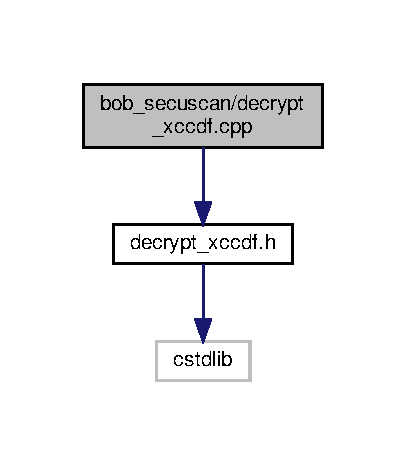
\includegraphics[width=195pt]{decrypt__xccdf_8cpp__incl}
\end{center}
\end{figure}
\subsection*{함수}
\begin{DoxyCompactItemize}
\item 
char $\ast$ \hyperlink{decrypt__xccdf_8cpp_a27469e936e25331c21909fd0c2c8baea}{decrypt} (int key, char $\ast$encrypted\+\_\+xml)
\end{DoxyCompactItemize}


\subsection{함수 문서화}
\mbox{\Hypertarget{decrypt__xccdf_8cpp_a27469e936e25331c21909fd0c2c8baea}\label{decrypt__xccdf_8cpp_a27469e936e25331c21909fd0c2c8baea}} 
\index{decrypt\+\_\+xccdf.\+cpp@{decrypt\+\_\+xccdf.\+cpp}!decrypt@{decrypt}}
\index{decrypt@{decrypt}!decrypt\+\_\+xccdf.\+cpp@{decrypt\+\_\+xccdf.\+cpp}}
\subsubsection{\texorpdfstring{decrypt()}{decrypt()}}
{\footnotesize\ttfamily char$\ast$ decrypt (\begin{DoxyParamCaption}\item[{int}]{key,  }\item[{char $\ast$}]{encrypted\+\_\+xml }\end{DoxyParamCaption})}

S\+H\+A256 Decode Function

decrypt(key, encrypted\+\_\+xml)

암호화 된 X\+ML 파일을 복호화 하는 함수를 정의합니다. 

decrypt\+\_\+xccdf.\+cpp 파일의 10 번째 라인에서 정의되었습니다.


\begin{DoxyCode}
10                                            \{
11     \textcolor{keywordtype}{char}* decrypted\_xml=(\textcolor{keywordtype}{char}*)malloc(\textcolor{keyword}{sizeof}(encrypted\_xml)/\textcolor{keyword}{sizeof}(char));
12     \textcolor{keywordflow}{return} sha256(key, encrypted\_xml);
13 \}
\end{DoxyCode}
이 함수를 호출하는 함수들에 대한 그래프입니다.\+:\nopagebreak
\begin{figure}[H]
\begin{center}
\leavevmode
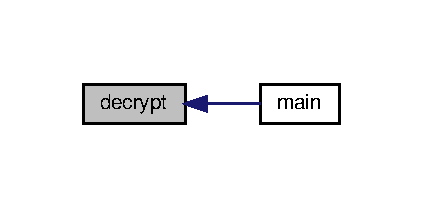
\includegraphics[width=203pt]{decrypt__xccdf_8cpp_a27469e936e25331c21909fd0c2c8baea_icgraph}
\end{center}
\end{figure}

\hypertarget{decrypt__xccdf_8h}{}\section{bob\+\_\+secuscan/decrypt\+\_\+xccdf.h 파일 참조}
\label{decrypt__xccdf_8h}\index{bob\+\_\+secuscan/decrypt\+\_\+xccdf.\+h@{bob\+\_\+secuscan/decrypt\+\_\+xccdf.\+h}}
{\ttfamily \#include $<$cstdlib$>$}\newline
decrypt\+\_\+xccdf.\+h에 대한 include 의존 그래프\nopagebreak
\begin{figure}[H]
\begin{center}
\leavevmode
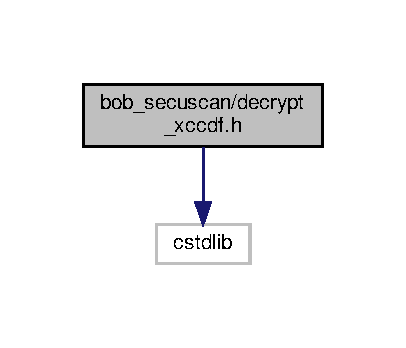
\includegraphics[width=195pt]{d0/deb/decrypt__xccdf_8h__incl}
\end{center}
\end{figure}
이 그래프는 이 파일을 직/간접적으로 include 하는 파일들을 보여줍니다.\+:\nopagebreak
\begin{figure}[H]
\begin{center}
\leavevmode
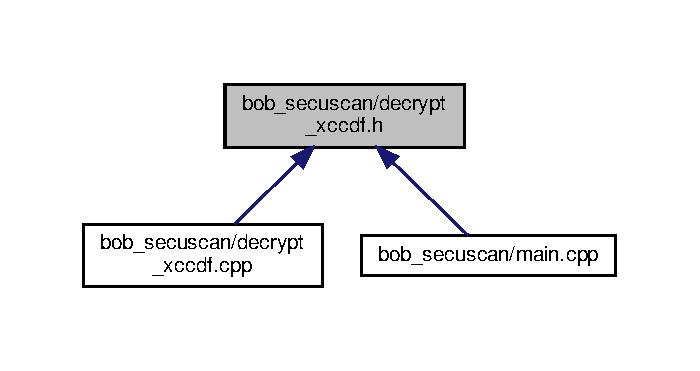
\includegraphics[width=336pt]{d1/d99/decrypt__xccdf_8h__dep__incl}
\end{center}
\end{figure}
\subsection*{함수}
\begin{DoxyCompactItemize}
\item 
char $\ast$ \hyperlink{decrypt__xccdf_8h_a27469e936e25331c21909fd0c2c8baea}{decrypt} (int key, char $\ast$encrypted\+\_\+xml)
\end{DoxyCompactItemize}


\subsection{함수 문서화}
\mbox{\Hypertarget{decrypt__xccdf_8h_a27469e936e25331c21909fd0c2c8baea}\label{decrypt__xccdf_8h_a27469e936e25331c21909fd0c2c8baea}} 
\index{decrypt\+\_\+xccdf.\+h@{decrypt\+\_\+xccdf.\+h}!decrypt@{decrypt}}
\index{decrypt@{decrypt}!decrypt\+\_\+xccdf.\+h@{decrypt\+\_\+xccdf.\+h}}
\subsubsection{\texorpdfstring{decrypt()}{decrypt()}}
{\footnotesize\ttfamily char$\ast$ decrypt (\begin{DoxyParamCaption}\item[{int}]{key,  }\item[{char $\ast$}]{encrypted\+\_\+xml }\end{DoxyParamCaption})}

decrypt\+\_\+xccdf.\+cpp에 사용하는 헤더 선언

S\+H\+A256 Decode Function

decrypt(key, encrypted\+\_\+xml)

암호화 된 X\+ML 파일을 복호화 하는 함수를 정의합니다. 

decrypt\+\_\+xccdf.\+cpp 파일의 10 번째 라인에서 정의되었습니다.

이 함수를 호출하는 함수들에 대한 그래프입니다.\+:\nopagebreak
\begin{figure}[H]
\begin{center}
\leavevmode
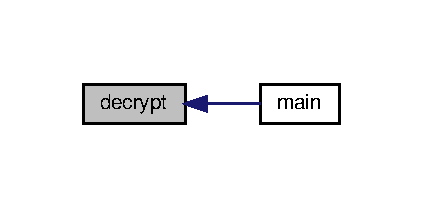
\includegraphics[width=203pt]{d0/dce/decrypt__xccdf_8h_a27469e936e25331c21909fd0c2c8baea_icgraph}
\end{center}
\end{figure}

\hypertarget{display_8cpp}{}\section{bob\+\_\+secuscan/display.cpp 파일 참조}
\label{display_8cpp}\index{bob\+\_\+secuscan/display.\+cpp@{bob\+\_\+secuscan/display.\+cpp}}
{\ttfamily \#include \char`\"{}display.\+h\char`\"{}}\newline
display.\+cpp에 대한 include 의존 그래프\nopagebreak
\begin{figure}[H]
\begin{center}
\leavevmode
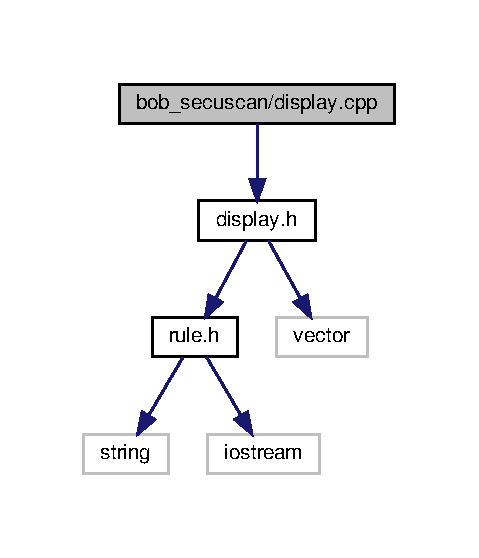
\includegraphics[width=230pt]{df/da5/display_8cpp__incl}
\end{center}
\end{figure}
\subsection*{함수}
\begin{DoxyCompactItemize}
\item 
void \hyperlink{display_8cpp_a97a370a188fd0a16b6577920ba34fd2c}{total\+\_\+check\+\_\+list} (vector$<$ \hyperlink{struct_rule}{Rule} $>$ \&ruleset, int $\ast$pf)
\item 
void \hyperlink{display_8cpp_aff64faf8c49787c8dabbd7eb2c4c2fdd}{show\+\_\+final\+\_\+score\+\_\+status} (int category)
\end{DoxyCompactItemize}


\subsection{함수 문서화}
\mbox{\Hypertarget{display_8cpp_aff64faf8c49787c8dabbd7eb2c4c2fdd}\label{display_8cpp_aff64faf8c49787c8dabbd7eb2c4c2fdd}} 
\index{display.\+cpp@{display.\+cpp}!show\+\_\+final\+\_\+score\+\_\+status@{show\+\_\+final\+\_\+score\+\_\+status}}
\index{show\+\_\+final\+\_\+score\+\_\+status@{show\+\_\+final\+\_\+score\+\_\+status}!display.\+cpp@{display.\+cpp}}
\subsubsection{\texorpdfstring{show\+\_\+final\+\_\+score\+\_\+status()}{show\_final\_score\_status()}}
{\footnotesize\ttfamily void show\+\_\+final\+\_\+score\+\_\+status (\begin{DoxyParamCaption}\item[{int}]{category }\end{DoxyParamCaption})}



display.\+cpp 파일의 14 번째 라인에서 정의되었습니다.

이 함수를 호출하는 함수들에 대한 그래프입니다.\+:\nopagebreak
\begin{figure}[H]
\begin{center}
\leavevmode
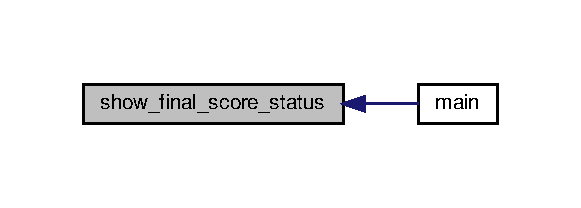
\includegraphics[width=279pt]{db/d86/display_8cpp_aff64faf8c49787c8dabbd7eb2c4c2fdd_icgraph}
\end{center}
\end{figure}
\mbox{\Hypertarget{display_8cpp_a97a370a188fd0a16b6577920ba34fd2c}\label{display_8cpp_a97a370a188fd0a16b6577920ba34fd2c}} 
\index{display.\+cpp@{display.\+cpp}!total\+\_\+check\+\_\+list@{total\+\_\+check\+\_\+list}}
\index{total\+\_\+check\+\_\+list@{total\+\_\+check\+\_\+list}!display.\+cpp@{display.\+cpp}}
\subsubsection{\texorpdfstring{total\+\_\+check\+\_\+list()}{total\_check\_list()}}
{\footnotesize\ttfamily void total\+\_\+check\+\_\+list (\begin{DoxyParamCaption}\item[{vector$<$ \hyperlink{struct_rule}{Rule} $>$ \&}]{ruleset,  }\item[{int $\ast$}]{pf }\end{DoxyParamCaption})}

점검 후에 체크리스트 디스플레이에 업데이트 할 수 있도록 total\+\_\+check\+\_\+list 를 선언해서 사용,

또한 최종 보고서 결과를 출력시키기 위해 show\+\_\+final\+\_\+score\+\_\+status 를 사용 

display.\+cpp 파일의 11 번째 라인에서 정의되었습니다.

이 함수를 호출하는 함수들에 대한 그래프입니다.\+:\nopagebreak
\begin{figure}[H]
\begin{center}
\leavevmode
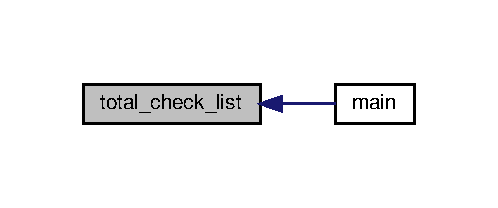
\includegraphics[width=239pt]{db/d86/display_8cpp_a97a370a188fd0a16b6577920ba34fd2c_icgraph}
\end{center}
\end{figure}

\hypertarget{display_8h}{}\section{bob\+\_\+secuscan/display.h 파일 참조}
\label{display_8h}\index{bob\+\_\+secuscan/display.\+h@{bob\+\_\+secuscan/display.\+h}}
{\ttfamily \#include \char`\"{}rule.\+h\char`\"{}}\newline
{\ttfamily \#include $<$vector$>$}\newline
display.\+h에 대한 include 의존 그래프\nopagebreak
\begin{figure}[H]
\begin{center}
\leavevmode
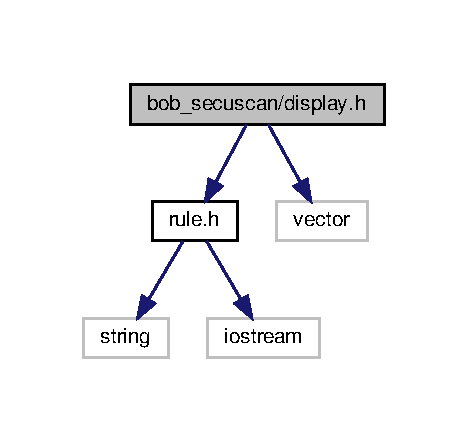
\includegraphics[width=225pt]{display_8h__incl}
\end{center}
\end{figure}
이 그래프는 이 파일을 직/간접적으로 include 하는 파일들을 보여줍니다.\+:\nopagebreak
\begin{figure}[H]
\begin{center}
\leavevmode
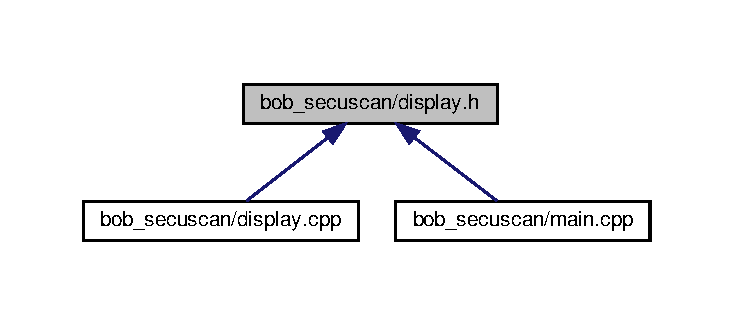
\includegraphics[width=350pt]{display_8h__dep__incl}
\end{center}
\end{figure}
\subsection*{함수}
\begin{DoxyCompactItemize}
\item 
void \hyperlink{display_8h_a97a370a188fd0a16b6577920ba34fd2c}{total\+\_\+check\+\_\+list} (vector$<$ \hyperlink{struct_rule}{Rule} $>$ \&ruleset, int $\ast$pf)
\item 
void \hyperlink{display_8h_aff64faf8c49787c8dabbd7eb2c4c2fdd}{show\+\_\+final\+\_\+score\+\_\+status} (int category)
\end{DoxyCompactItemize}


\subsection{함수 문서화}
\mbox{\Hypertarget{display_8h_aff64faf8c49787c8dabbd7eb2c4c2fdd}\label{display_8h_aff64faf8c49787c8dabbd7eb2c4c2fdd}} 
\index{display.\+h@{display.\+h}!show\+\_\+final\+\_\+score\+\_\+status@{show\+\_\+final\+\_\+score\+\_\+status}}
\index{show\+\_\+final\+\_\+score\+\_\+status@{show\+\_\+final\+\_\+score\+\_\+status}!display.\+h@{display.\+h}}
\subsubsection{\texorpdfstring{show\+\_\+final\+\_\+score\+\_\+status()}{show\_final\_score\_status()}}
{\footnotesize\ttfamily void show\+\_\+final\+\_\+score\+\_\+status (\begin{DoxyParamCaption}\item[{int}]{category }\end{DoxyParamCaption})}

보고서 output 

display.\+cpp 파일의 6 번째 라인에서 정의되었습니다.


\begin{DoxyCode}
6                                           \{
7 
8 \}
\end{DoxyCode}
이 함수를 호출하는 함수들에 대한 그래프입니다.\+:\nopagebreak
\begin{figure}[H]
\begin{center}
\leavevmode
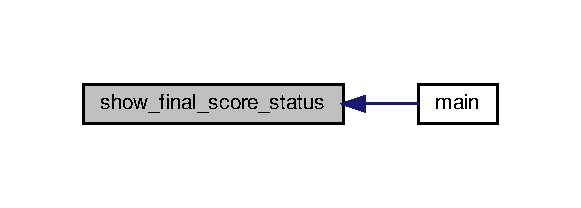
\includegraphics[width=279pt]{display_8h_aff64faf8c49787c8dabbd7eb2c4c2fdd_icgraph}
\end{center}
\end{figure}
\mbox{\Hypertarget{display_8h_a97a370a188fd0a16b6577920ba34fd2c}\label{display_8h_a97a370a188fd0a16b6577920ba34fd2c}} 
\index{display.\+h@{display.\+h}!total\+\_\+check\+\_\+list@{total\+\_\+check\+\_\+list}}
\index{total\+\_\+check\+\_\+list@{total\+\_\+check\+\_\+list}!display.\+h@{display.\+h}}
\subsubsection{\texorpdfstring{total\+\_\+check\+\_\+list()}{total\_check\_list()}}
{\footnotesize\ttfamily void total\+\_\+check\+\_\+list (\begin{DoxyParamCaption}\item[{vector$<$ \hyperlink{struct_rule}{Rule} $>$ \&}]{ruleset,  }\item[{int $\ast$}]{pf }\end{DoxyParamCaption})}

검사 후 체크리스트 디스플레이에 업데이트 

display.\+cpp 파일의 3 번째 라인에서 정의되었습니다.


\begin{DoxyCode}
3                                                      \{
4 \}
\end{DoxyCode}
이 함수를 호출하는 함수들에 대한 그래프입니다.\+:\nopagebreak
\begin{figure}[H]
\begin{center}
\leavevmode
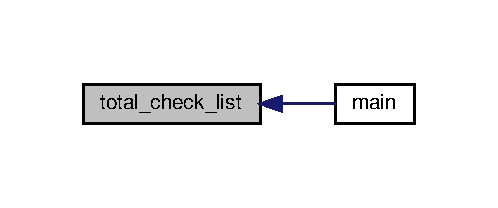
\includegraphics[width=239pt]{display_8h_a97a370a188fd0a16b6577920ba34fd2c_icgraph}
\end{center}
\end{figure}

\hypertarget{engine_8cpp}{}\section{bob\+\_\+secuscan/engine.cpp 파일 참조}
\label{engine_8cpp}\index{bob\+\_\+secuscan/engine.\+cpp@{bob\+\_\+secuscan/engine.\+cpp}}
{\ttfamily \#include \char`\"{}engine.\+h\char`\"{}}\newline
engine.\+cpp에 대한 include 의존 그래프\nopagebreak
\begin{figure}[H]
\begin{center}
\leavevmode
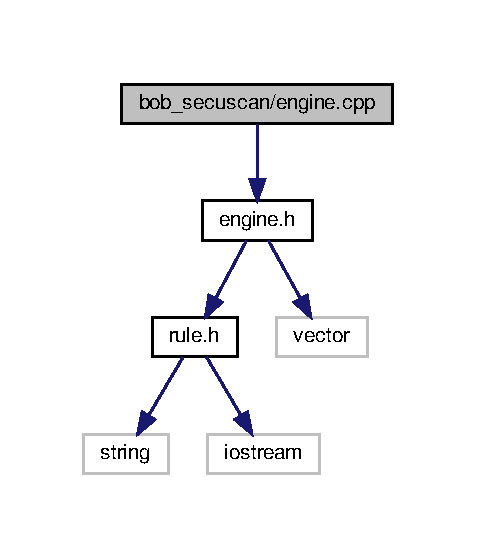
\includegraphics[width=229pt]{engine_8cpp__incl}
\end{center}
\end{figure}
\subsection*{함수}
\begin{DoxyCompactItemize}
\item 
int $\ast$ \hyperlink{engine_8cpp_ad5b63e5aa719dc0a51ea42c29a5c921a}{exec\+\_\+engine} (vector$<$ \hyperlink{struct_rule}{Rule} $>$ \&ruleset, int $\ast$pf)
\item 
int \hyperlink{engine_8cpp_aa6f727915aba330716bbe1bf16f898e2}{check\+\_\+regex} ()
\item 
int \hyperlink{engine_8cpp_a9593c4e9695af7b9c8de6d4295ed41b2}{check\+\_\+authority} ()
\item 
void \hyperlink{engine_8cpp_a0f15a8265e6f3a4a16da1286c6659721}{fixation} (\hyperlink{struct_rule}{Rule} rule)
\end{DoxyCompactItemize}


\subsection{함수 문서화}
\mbox{\Hypertarget{engine_8cpp_a9593c4e9695af7b9c8de6d4295ed41b2}\label{engine_8cpp_a9593c4e9695af7b9c8de6d4295ed41b2}} 
\index{engine.\+cpp@{engine.\+cpp}!check\+\_\+authority@{check\+\_\+authority}}
\index{check\+\_\+authority@{check\+\_\+authority}!engine.\+cpp@{engine.\+cpp}}
\subsubsection{\texorpdfstring{check\+\_\+authority()}{check\_authority()}}
{\footnotesize\ttfamily int check\+\_\+authority (\begin{DoxyParamCaption}{ }\end{DoxyParamCaption})}

루트 권한 체크 루트 권한 체크 

engine.\+cpp 파일의 21 번째 라인에서 정의되었습니다.


\begin{DoxyCode}
21                      \{
23 \}
\end{DoxyCode}
이 함수를 호출하는 함수들에 대한 그래프입니다.\+:\nopagebreak
\begin{figure}[H]
\begin{center}
\leavevmode
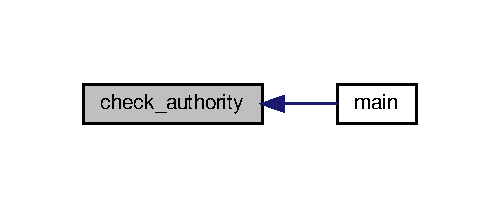
\includegraphics[width=240pt]{engine_8cpp_a9593c4e9695af7b9c8de6d4295ed41b2_icgraph}
\end{center}
\end{figure}
\mbox{\Hypertarget{engine_8cpp_aa6f727915aba330716bbe1bf16f898e2}\label{engine_8cpp_aa6f727915aba330716bbe1bf16f898e2}} 
\index{engine.\+cpp@{engine.\+cpp}!check\+\_\+regex@{check\+\_\+regex}}
\index{check\+\_\+regex@{check\+\_\+regex}!engine.\+cpp@{engine.\+cpp}}
\subsubsection{\texorpdfstring{check\+\_\+regex()}{check\_regex()}}
{\footnotesize\ttfamily int check\+\_\+regex (\begin{DoxyParamCaption}{ }\end{DoxyParamCaption})}

정규표현식 여부 검사 정규표현식 여부 검사 

engine.\+cpp 파일의 17 번째 라인에서 정의되었습니다.


\begin{DoxyCode}
17                  \{
19 \}
\end{DoxyCode}
이 함수를 호출하는 함수들에 대한 그래프입니다.\+:\nopagebreak
\begin{figure}[H]
\begin{center}
\leavevmode
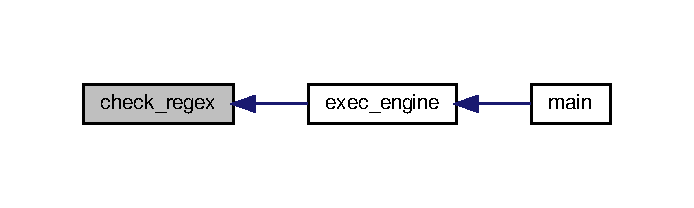
\includegraphics[width=333pt]{engine_8cpp_aa6f727915aba330716bbe1bf16f898e2_icgraph}
\end{center}
\end{figure}
\mbox{\Hypertarget{engine_8cpp_ad5b63e5aa719dc0a51ea42c29a5c921a}\label{engine_8cpp_ad5b63e5aa719dc0a51ea42c29a5c921a}} 
\index{engine.\+cpp@{engine.\+cpp}!exec\+\_\+engine@{exec\+\_\+engine}}
\index{exec\+\_\+engine@{exec\+\_\+engine}!engine.\+cpp@{engine.\+cpp}}
\subsubsection{\texorpdfstring{exec\+\_\+engine()}{exec\_engine()}}
{\footnotesize\ttfamily int$\ast$ exec\+\_\+engine (\begin{DoxyParamCaption}\item[{vector$<$ \hyperlink{struct_rule}{Rule} $>$ \&}]{ruleset,  }\item[{int $\ast$}]{pf }\end{DoxyParamCaption})}

검사 수행 엔진 정규식 검사 

engine.\+cpp 파일의 3 번째 라인에서 정의되었습니다.


\begin{DoxyCode}
3                                                 \{
4     \textcolor{keywordtype}{int} passfail[200];
5     vector<Rule>::iterator ptr;
6     \textcolor{keywordflow}{for}(ptr=ruleset.begin(); ptr!=ruleset.end(); ptr++)\{
7         \textcolor{keywordflow}{if}(\hyperlink{engine_8cpp_aa6f727915aba330716bbe1bf16f898e2}{check\_regex}())\{
9         \}
10         \textcolor{keywordflow}{else}\{
11             system(ptr->test);
12         \}
13     \}
14     \textcolor{keywordflow}{return} passfail;
15 \}
\end{DoxyCode}
이 함수 내부에서 호출하는 함수들에 대한 그래프입니다.\+:\nopagebreak
\begin{figure}[H]
\begin{center}
\leavevmode
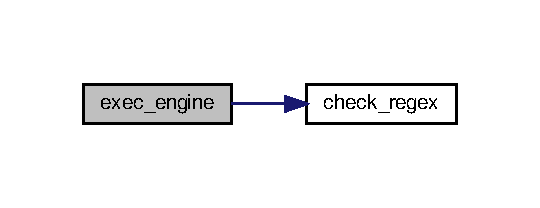
\includegraphics[width=259pt]{engine_8cpp_ad5b63e5aa719dc0a51ea42c29a5c921a_cgraph}
\end{center}
\end{figure}
이 함수를 호출하는 함수들에 대한 그래프입니다.\+:\nopagebreak
\begin{figure}[H]
\begin{center}
\leavevmode
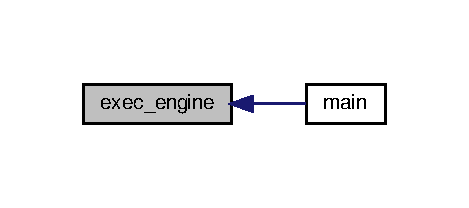
\includegraphics[width=225pt]{engine_8cpp_ad5b63e5aa719dc0a51ea42c29a5c921a_icgraph}
\end{center}
\end{figure}
\mbox{\Hypertarget{engine_8cpp_a0f15a8265e6f3a4a16da1286c6659721}\label{engine_8cpp_a0f15a8265e6f3a4a16da1286c6659721}} 
\index{engine.\+cpp@{engine.\+cpp}!fixation@{fixation}}
\index{fixation@{fixation}!engine.\+cpp@{engine.\+cpp}}
\subsubsection{\texorpdfstring{fixation()}{fixation()}}
{\footnotesize\ttfamily void fixation (\begin{DoxyParamCaption}\item[{\hyperlink{struct_rule}{Rule}}]{rule }\end{DoxyParamCaption})}

fix 수행 fix 수행 

engine.\+cpp 파일의 25 번째 라인에서 정의되었습니다.


\begin{DoxyCode}
25                         \{
27 \}
\end{DoxyCode}
이 함수를 호출하는 함수들에 대한 그래프입니다.\+:\nopagebreak
\begin{figure}[H]
\begin{center}
\leavevmode
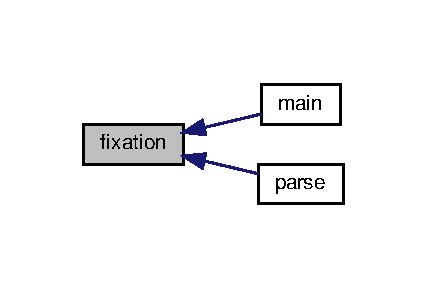
\includegraphics[width=205pt]{engine_8cpp_a0f15a8265e6f3a4a16da1286c6659721_icgraph}
\end{center}
\end{figure}

\hypertarget{engine_8h}{}\section{bob\+\_\+secuscan/engine.h 파일 참조}
\label{engine_8h}\index{bob\+\_\+secuscan/engine.\+h@{bob\+\_\+secuscan/engine.\+h}}
{\ttfamily \#include \char`\"{}rule.\+h\char`\"{}}\newline
{\ttfamily \#include $<$vector$>$}\newline
engine.\+h에 대한 include 의존 그래프
\nopagebreak
\begin{figure}[H]
\begin{center}
\leavevmode
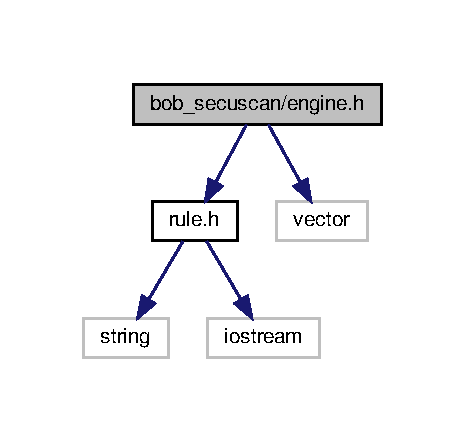
\includegraphics[width=223pt]{engine_8h__incl}
\end{center}
\end{figure}
이 그래프는 이 파일을 직/간접적으로 include 하는 파일들을 보여줍니다.\+:
\nopagebreak
\begin{figure}[H]
\begin{center}
\leavevmode
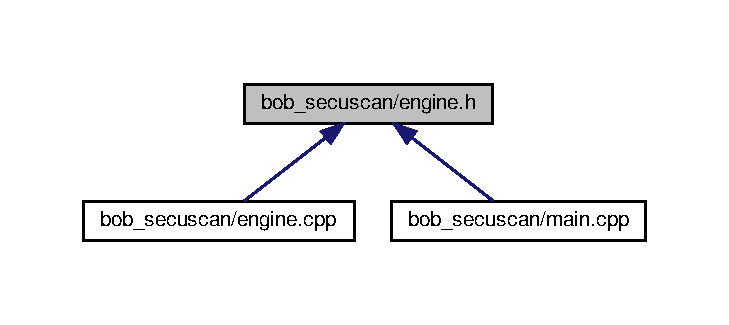
\includegraphics[width=350pt]{engine_8h__dep__incl}
\end{center}
\end{figure}
\subsection*{함수}
\begin{DoxyCompactItemize}
\item 
int $\ast$ \hyperlink{engine_8h_ad5b63e5aa719dc0a51ea42c29a5c921a}{exec\+\_\+engine} (vector$<$ \hyperlink{struct_rule}{Rule} $>$ \&ruleset, int $\ast$pf)
\item 
int \hyperlink{engine_8h_aa6f727915aba330716bbe1bf16f898e2}{check\+\_\+regex} ()
\item 
int \hyperlink{engine_8h_a9593c4e9695af7b9c8de6d4295ed41b2}{check\+\_\+authority} ()
\item 
void \hyperlink{engine_8h_a0f15a8265e6f3a4a16da1286c6659721}{fixation} (\hyperlink{struct_rule}{Rule} rule)
\end{DoxyCompactItemize}


\subsection{함수 문서화}
\mbox{\Hypertarget{engine_8h_a9593c4e9695af7b9c8de6d4295ed41b2}\label{engine_8h_a9593c4e9695af7b9c8de6d4295ed41b2}} 
\index{engine.\+h@{engine.\+h}!check\+\_\+authority@{check\+\_\+authority}}
\index{check\+\_\+authority@{check\+\_\+authority}!engine.\+h@{engine.\+h}}
\subsubsection{\texorpdfstring{check\+\_\+authority()}{check\_authority()}}
{\footnotesize\ttfamily int check\+\_\+authority (\begin{DoxyParamCaption}{ }\end{DoxyParamCaption})}

루트 권한 체크 루트 권한 체크 

engine.\+cpp 파일의 21 번째 라인에서 정의되었습니다.


\begin{DoxyCode}
21                      \{
23 \}
\end{DoxyCode}
이 함수를 호출하는 함수들에 대한 그래프입니다.\+:
\nopagebreak
\begin{figure}[H]
\begin{center}
\leavevmode
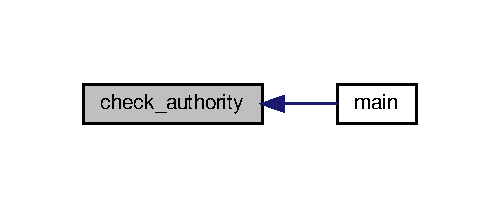
\includegraphics[width=240pt]{engine_8h_a9593c4e9695af7b9c8de6d4295ed41b2_icgraph}
\end{center}
\end{figure}
\mbox{\Hypertarget{engine_8h_aa6f727915aba330716bbe1bf16f898e2}\label{engine_8h_aa6f727915aba330716bbe1bf16f898e2}} 
\index{engine.\+h@{engine.\+h}!check\+\_\+regex@{check\+\_\+regex}}
\index{check\+\_\+regex@{check\+\_\+regex}!engine.\+h@{engine.\+h}}
\subsubsection{\texorpdfstring{check\+\_\+regex()}{check\_regex()}}
{\footnotesize\ttfamily int check\+\_\+regex (\begin{DoxyParamCaption}{ }\end{DoxyParamCaption})}

정규표현식 여부 검사 정규표현식 여부 검사 

engine.\+cpp 파일의 17 번째 라인에서 정의되었습니다.


\begin{DoxyCode}
17                  \{
19 \}
\end{DoxyCode}
이 함수를 호출하는 함수들에 대한 그래프입니다.\+:
\nopagebreak
\begin{figure}[H]
\begin{center}
\leavevmode
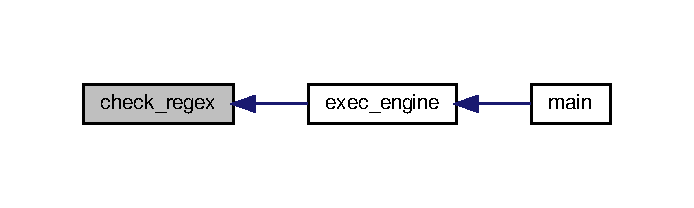
\includegraphics[width=333pt]{engine_8h_aa6f727915aba330716bbe1bf16f898e2_icgraph}
\end{center}
\end{figure}
\mbox{\Hypertarget{engine_8h_ad5b63e5aa719dc0a51ea42c29a5c921a}\label{engine_8h_ad5b63e5aa719dc0a51ea42c29a5c921a}} 
\index{engine.\+h@{engine.\+h}!exec\+\_\+engine@{exec\+\_\+engine}}
\index{exec\+\_\+engine@{exec\+\_\+engine}!engine.\+h@{engine.\+h}}
\subsubsection{\texorpdfstring{exec\+\_\+engine()}{exec\_engine()}}
{\footnotesize\ttfamily int$\ast$ exec\+\_\+engine (\begin{DoxyParamCaption}\item[{vector$<$ \hyperlink{struct_rule}{Rule} $>$ \&}]{ruleset,  }\item[{int $\ast$}]{pf }\end{DoxyParamCaption})}

검사 수행 엔진 정규식 검사 

engine.\+cpp 파일의 3 번째 라인에서 정의되었습니다.


\begin{DoxyCode}
3                                                 \{
4     \textcolor{keywordtype}{int} passfail[200];
5     vector<Rule>::iterator ptr;
6     \textcolor{keywordflow}{for}(ptr=ruleset.begin(); ptr!=ruleset.end(); ptr++)\{
7         \textcolor{keywordflow}{if}(\hyperlink{engine_8cpp_aa6f727915aba330716bbe1bf16f898e2}{check\_regex}())\{
9         \}
10         \textcolor{keywordflow}{else}\{
11             system(ptr->test);
12         \}
13     \}
14     \textcolor{keywordflow}{return} passfail;
15 \}
\end{DoxyCode}
이 함수 내부에서 호출하는 함수들에 대한 그래프입니다.\+:
\nopagebreak
\begin{figure}[H]
\begin{center}
\leavevmode
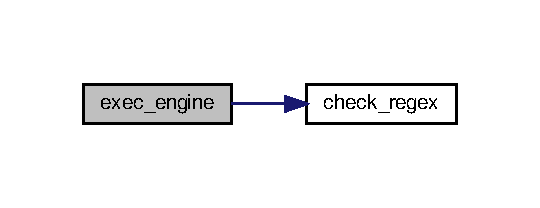
\includegraphics[width=259pt]{engine_8h_ad5b63e5aa719dc0a51ea42c29a5c921a_cgraph}
\end{center}
\end{figure}
이 함수를 호출하는 함수들에 대한 그래프입니다.\+:
\nopagebreak
\begin{figure}[H]
\begin{center}
\leavevmode
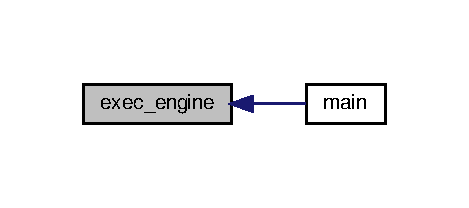
\includegraphics[width=225pt]{engine_8h_ad5b63e5aa719dc0a51ea42c29a5c921a_icgraph}
\end{center}
\end{figure}
\mbox{\Hypertarget{engine_8h_a0f15a8265e6f3a4a16da1286c6659721}\label{engine_8h_a0f15a8265e6f3a4a16da1286c6659721}} 
\index{engine.\+h@{engine.\+h}!fixation@{fixation}}
\index{fixation@{fixation}!engine.\+h@{engine.\+h}}
\subsubsection{\texorpdfstring{fixation()}{fixation()}}
{\footnotesize\ttfamily void fixation (\begin{DoxyParamCaption}\item[{\hyperlink{struct_rule}{Rule}}]{rule }\end{DoxyParamCaption})}

fix 수행 fix 수행 

engine.\+cpp 파일의 25 번째 라인에서 정의되었습니다.


\begin{DoxyCode}
25                         \{
27 \}
\end{DoxyCode}
이 함수를 호출하는 함수들에 대한 그래프입니다.\+:
\nopagebreak
\begin{figure}[H]
\begin{center}
\leavevmode
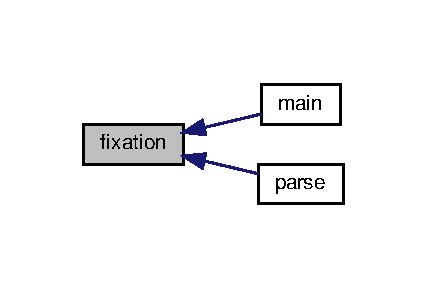
\includegraphics[width=205pt]{engine_8h_a0f15a8265e6f3a4a16da1286c6659721_icgraph}
\end{center}
\end{figure}

\hypertarget{html__report_8cpp}{}\section{bob\+\_\+secuscan/html\+\_\+report.cpp 파일 참조}
\label{html__report_8cpp}\index{bob\+\_\+secuscan/html\+\_\+report.\+cpp@{bob\+\_\+secuscan/html\+\_\+report.\+cpp}}
{\ttfamily \#include \char`\"{}html\+\_\+report.\+h\char`\"{}}\newline
html\+\_\+report.\+cpp에 대한 include 의존 그래프
\nopagebreak
\begin{figure}[H]
\begin{center}
\leavevmode
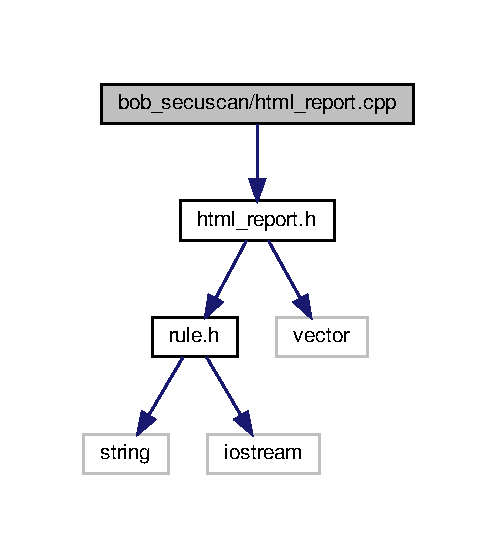
\includegraphics[width=239pt]{html__report_8cpp__incl}
\end{center}
\end{figure}
\subsection*{함수}
\begin{DoxyCompactItemize}
\item 
void \hyperlink{html__report_8cpp_a202d1a90bd705341eb39c7e744c86516}{create\+\_\+html} (vector$<$ \hyperlink{struct_rule}{Rule} $>$ \&ruleset, int $\ast$pf)
\end{DoxyCompactItemize}


\subsection{함수 문서화}
\mbox{\Hypertarget{html__report_8cpp_a202d1a90bd705341eb39c7e744c86516}\label{html__report_8cpp_a202d1a90bd705341eb39c7e744c86516}} 
\index{html\+\_\+report.\+cpp@{html\+\_\+report.\+cpp}!create\+\_\+html@{create\+\_\+html}}
\index{create\+\_\+html@{create\+\_\+html}!html\+\_\+report.\+cpp@{html\+\_\+report.\+cpp}}
\subsubsection{\texorpdfstring{create\+\_\+html()}{create\_html()}}
{\footnotesize\ttfamily void create\+\_\+html (\begin{DoxyParamCaption}\item[{vector$<$ \hyperlink{struct_rule}{Rule} $>$ \&}]{ruleset,  }\item[{int $\ast$}]{pf }\end{DoxyParamCaption})}

html report 생성 

html\+\_\+report.\+cpp 파일의 3 번째 라인에서 정의되었습니다.


\begin{DoxyCode}
3                                                 \{
4 
5 \}
\end{DoxyCode}
이 함수를 호출하는 함수들에 대한 그래프입니다.\+:
\nopagebreak
\begin{figure}[H]
\begin{center}
\leavevmode
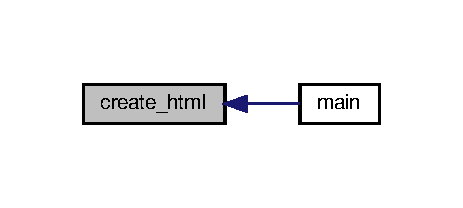
\includegraphics[width=222pt]{html__report_8cpp_a202d1a90bd705341eb39c7e744c86516_icgraph}
\end{center}
\end{figure}

\hypertarget{html__report_8h}{}\section{bob\+\_\+secuscan/html\+\_\+report.h 파일 참조}
\label{html__report_8h}\index{bob\+\_\+secuscan/html\+\_\+report.\+h@{bob\+\_\+secuscan/html\+\_\+report.\+h}}
{\ttfamily \#include \char`\"{}rule.\+h\char`\"{}}\newline
{\ttfamily \#include $<$vector$>$}\newline
html\+\_\+report.\+h에 대한 include 의존 그래프\nopagebreak
\begin{figure}[H]
\begin{center}
\leavevmode
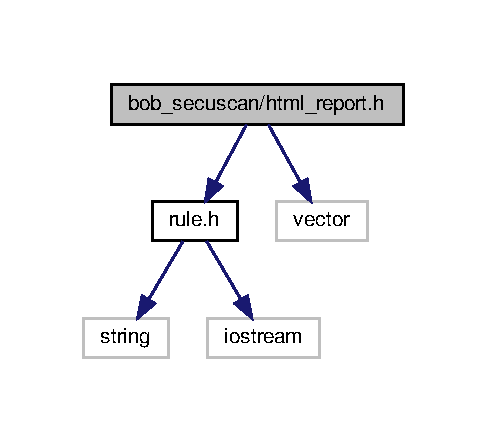
\includegraphics[width=234pt]{html__report_8h__incl}
\end{center}
\end{figure}
이 그래프는 이 파일을 직/간접적으로 include 하는 파일들을 보여줍니다.\+:\nopagebreak
\begin{figure}[H]
\begin{center}
\leavevmode
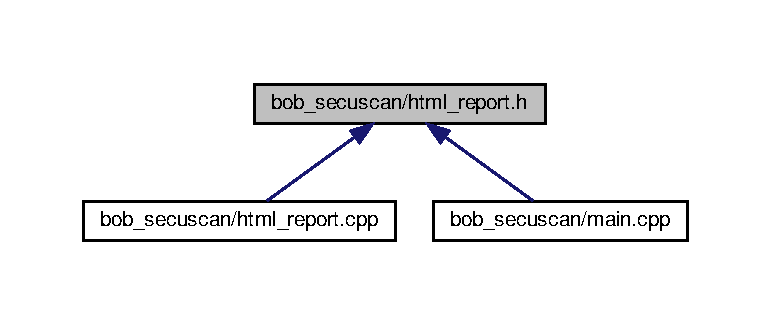
\includegraphics[width=350pt]{html__report_8h__dep__incl}
\end{center}
\end{figure}
\subsection*{함수}
\begin{DoxyCompactItemize}
\item 
void \hyperlink{html__report_8h_a202d1a90bd705341eb39c7e744c86516}{create\+\_\+html} (vector$<$ \hyperlink{struct_rule}{Rule} $>$ \&ruleset, int $\ast$pf)
\end{DoxyCompactItemize}


\subsection{함수 문서화}
\mbox{\Hypertarget{html__report_8h_a202d1a90bd705341eb39c7e744c86516}\label{html__report_8h_a202d1a90bd705341eb39c7e744c86516}} 
\index{html\+\_\+report.\+h@{html\+\_\+report.\+h}!create\+\_\+html@{create\+\_\+html}}
\index{create\+\_\+html@{create\+\_\+html}!html\+\_\+report.\+h@{html\+\_\+report.\+h}}
\subsubsection{\texorpdfstring{create\+\_\+html()}{create\_html()}}
{\footnotesize\ttfamily void create\+\_\+html (\begin{DoxyParamCaption}\item[{vector$<$ \hyperlink{struct_rule}{Rule} $>$ \&}]{ruleset,  }\item[{int $\ast$}]{pf }\end{DoxyParamCaption})}

html report 생성 

html\+\_\+report.\+cpp 파일의 3 번째 라인에서 정의되었습니다.


\begin{DoxyCode}
3                                                 \{
4 
5 \}
\end{DoxyCode}
이 함수를 호출하는 함수들에 대한 그래프입니다.\+:\nopagebreak
\begin{figure}[H]
\begin{center}
\leavevmode
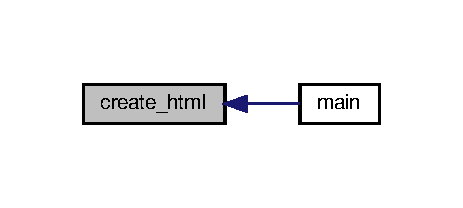
\includegraphics[width=222pt]{html__report_8h_a202d1a90bd705341eb39c7e744c86516_icgraph}
\end{center}
\end{figure}

\hypertarget{main_8cpp}{}\section{bob\+\_\+secuscan/main.cpp 파일 참조}
\label{main_8cpp}\index{bob\+\_\+secuscan/main.\+cpp@{bob\+\_\+secuscan/main.\+cpp}}
{\ttfamily \#include $<$cstdio$>$}\newline
{\ttfamily \#include $<$cstdlib$>$}\newline
{\ttfamily \#include $<$vector$>$}\newline
{\ttfamily \#include \char`\"{}rule.\+h\char`\"{}}\newline
{\ttfamily \#include \char`\"{}decrypt\+\_\+xccdf.\+h\char`\"{}}\newline
{\ttfamily \#include \char`\"{}xml\+\_\+parser.\+h\char`\"{}}\newline
{\ttfamily \#include \char`\"{}engine.\+h\char`\"{}}\newline
{\ttfamily \#include \char`\"{}scoring.\+h\char`\"{}}\newline
{\ttfamily \#include \char`\"{}display.\+h\char`\"{}}\newline
{\ttfamily \#include \char`\"{}pdf\+\_\+report.\+h\char`\"{}}\newline
{\ttfamily \#include \char`\"{}html\+\_\+report.\+h\char`\"{}}\newline
main.\+cpp에 대한 include 의존 그래프\nopagebreak
\begin{figure}[H]
\begin{center}
\leavevmode
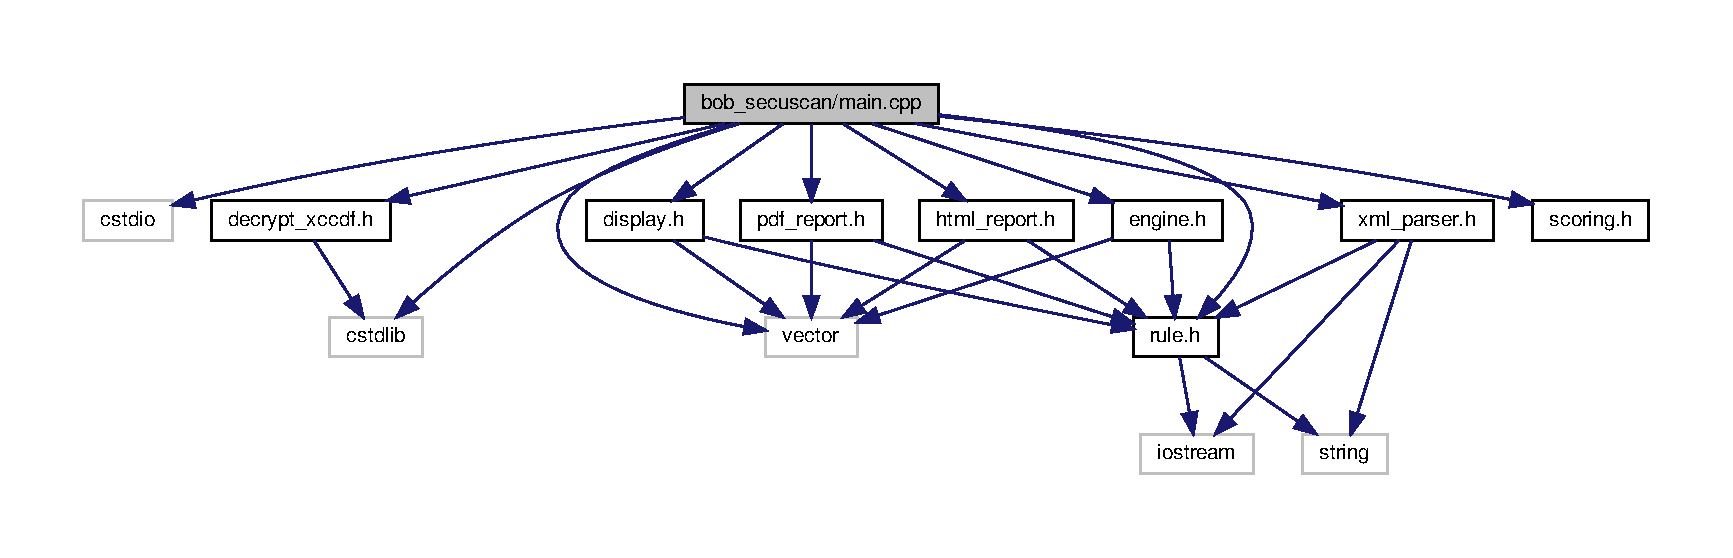
\includegraphics[width=350pt]{main_8cpp__incl}
\end{center}
\end{figure}
\subsection*{매크로}
\begin{DoxyCompactItemize}
\item 
\#define \hyperlink{main_8cpp_ae3121841e645911456fe29d422b320e9}{H\+T\+ML}~1
\item 
\#define \hyperlink{main_8cpp_a50a6a866f6648822f5f99cba121bbd35}{P\+DF}~2
\end{DoxyCompactItemize}
\subsection*{함수}
\begin{DoxyCompactItemize}
\item 
int \hyperlink{main_8cpp_ae66f6b31b5ad750f1fe042a706a4e3d4}{main} ()
\end{DoxyCompactItemize}


\subsection{매크로 문서화}
\mbox{\Hypertarget{main_8cpp_ae3121841e645911456fe29d422b320e9}\label{main_8cpp_ae3121841e645911456fe29d422b320e9}} 
\index{main.\+cpp@{main.\+cpp}!H\+T\+ML@{H\+T\+ML}}
\index{H\+T\+ML@{H\+T\+ML}!main.\+cpp@{main.\+cpp}}
\subsubsection{\texorpdfstring{H\+T\+ML}{HTML}}
{\footnotesize\ttfamily \#define H\+T\+ML~1}



main.\+cpp 파일의 12 번째 라인에서 정의되었습니다.

\mbox{\Hypertarget{main_8cpp_a50a6a866f6648822f5f99cba121bbd35}\label{main_8cpp_a50a6a866f6648822f5f99cba121bbd35}} 
\index{main.\+cpp@{main.\+cpp}!P\+DF@{P\+DF}}
\index{P\+DF@{P\+DF}!main.\+cpp@{main.\+cpp}}
\subsubsection{\texorpdfstring{P\+DF}{PDF}}
{\footnotesize\ttfamily \#define P\+DF~2}



main.\+cpp 파일의 13 번째 라인에서 정의되었습니다.



\subsection{함수 문서화}
\mbox{\Hypertarget{main_8cpp_ae66f6b31b5ad750f1fe042a706a4e3d4}\label{main_8cpp_ae66f6b31b5ad750f1fe042a706a4e3d4}} 
\index{main.\+cpp@{main.\+cpp}!main@{main}}
\index{main@{main}!main.\+cpp@{main.\+cpp}}
\subsubsection{\texorpdfstring{main()}{main()}}
{\footnotesize\ttfamily int main (\begin{DoxyParamCaption}{ }\end{DoxyParamCaption})}

암호화된 xccdf 파일 읽기

sha256 decryption

parsing rules

루트인지 권한 체크

cvss scoring 

main.\+cpp 파일의 14 번째 라인에서 정의되었습니다.


\begin{DoxyCode}
14           \{
16     FILE *file = fopen(\textcolor{stringliteral}{"xccdf\_sample.xml"} , \textcolor{stringliteral}{"rb"});
17     \textcolor{keywordtype}{char} xml\_binary[200];
18     \textcolor{keywordflow}{if} (file == NULL) \{ printf(\textcolor{stringliteral}{"파일을 읽기 모드로 열 수 없습니다.\(\backslash\)n"});
19         \textcolor{keywordflow}{return} 0; 
20     \}
21     fread(xml\_binary , \textcolor{keyword}{sizeof}(xml\_binary) , 1 , file);
22     fclose(file);
24     \textcolor{keywordtype}{char}* decrypted\_xml=\hyperlink{decrypt__xccdf_8cpp_a27469e936e25331c21909fd0c2c8baea}{decrypt}(PRIVATE\_KEY, xml\_binary);
26     vector<Rule> rule\_set;
27     \textcolor{keywordflow}{for}(\textcolor{keywordtype}{int} i=0; i<line; i++)\{
28         \hyperlink{struct_rule}{Rule} temp=decrypted\_xml[i];
29         rule\_set.push\_back(temp);
30     \}
31     \textcolor{keywordtype}{int} passfail[200];
33     \textcolor{keywordflow}{if}(!\hyperlink{engine_8cpp_a9593c4e9695af7b9c8de6d4295ed41b2}{check\_authority}())\{
34         printf(\textcolor{stringliteral}{"no authority!\(\backslash\)n"});
35         exit(0);
36     \}
37     memcpy(passfail, \hyperlink{engine_8cpp_ad5b63e5aa719dc0a51ea42c29a5c921a}{exec\_engine}(rule\_set, passfail), \textcolor{keyword}{sizeof}(passfail));
39     \hyperlink{scoring_8cpp_afc65323578d43d64369eeeb29a163376}{cvss\_score}(passfail);
40     \hyperlink{display_8cpp_a97a370a188fd0a16b6577920ba34fd2c}{total\_check\_list}(rule\_set, passfail);
41     \textcolor{keywordtype}{int} response;
42     \textcolor{keywordflow}{while}(response=on\_click(Save\_button))\{
43         \textcolor{keywordflow}{if}(on\_click(Result.fix))\{
44             \hyperlink{engine_8cpp_a0f15a8265e6f3a4a16da1286c6659721}{fixation}(rule\_set[Result.index()]);
45         \}
46     \}
47     \hyperlink{html__report_8cpp_a202d1a90bd705341eb39c7e744c86516}{create\_html}(rule\_set, passfail);
48     \hyperlink{pdf__report_8cpp_a9a68b1bf8ea084181a40a5296be9d805}{create\_pdf}(rule\_set, passfail);
49     \textcolor{keywordflow}{switch} (modify\_category(response))
50     \{
51     \textcolor{keywordflow}{case} \hyperlink{main_8cpp_ae3121841e645911456fe29d422b320e9}{HTML}:
52         \hyperlink{display_8cpp_aff64faf8c49787c8dabbd7eb2c4c2fdd}{show\_final\_score\_status}(\hyperlink{main_8cpp_ae3121841e645911456fe29d422b320e9}{HTML});
53         \textcolor{keywordflow}{break};
54     \textcolor{keywordflow}{case} \hyperlink{main_8cpp_a50a6a866f6648822f5f99cba121bbd35}{PDF}:
55         \hyperlink{display_8cpp_aff64faf8c49787c8dabbd7eb2c4c2fdd}{show\_final\_score\_status}(\hyperlink{main_8cpp_a50a6a866f6648822f5f99cba121bbd35}{PDF});
56         \textcolor{keywordflow}{break};
57     \textcolor{keywordflow}{default}:
58         \textcolor{keywordflow}{break};
59     \}
60     \textcolor{keywordflow}{return} 0;
61 \}
\end{DoxyCode}
이 함수 내부에서 호출하는 함수들에 대한 그래프입니다.\+:\nopagebreak
\begin{figure}[H]
\begin{center}
\leavevmode
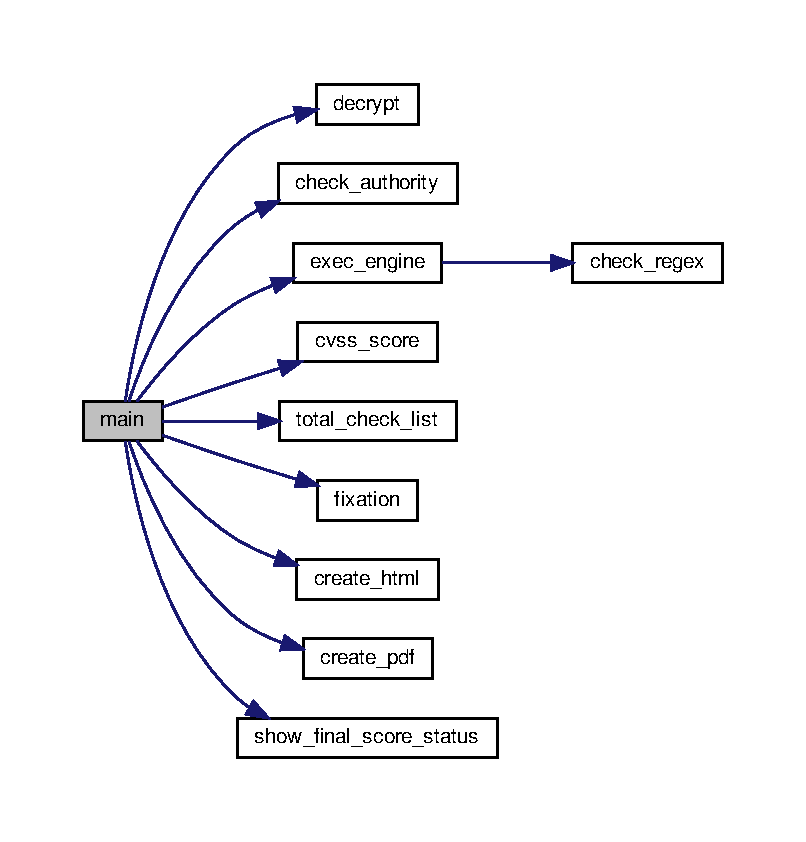
\includegraphics[width=350pt]{main_8cpp_ae66f6b31b5ad750f1fe042a706a4e3d4_cgraph}
\end{center}
\end{figure}

\hypertarget{pdf__report_8cpp}{}\section{bob\+\_\+secuscan/pdf\+\_\+report.cpp 파일 참조}
\label{pdf__report_8cpp}\index{bob\+\_\+secuscan/pdf\+\_\+report.\+cpp@{bob\+\_\+secuscan/pdf\+\_\+report.\+cpp}}
{\ttfamily \#include \char`\"{}pdf\+\_\+report.\+h\char`\"{}}\newline
pdf\+\_\+report.\+cpp에 대한 include 의존 그래프\nopagebreak
\begin{figure}[H]
\begin{center}
\leavevmode
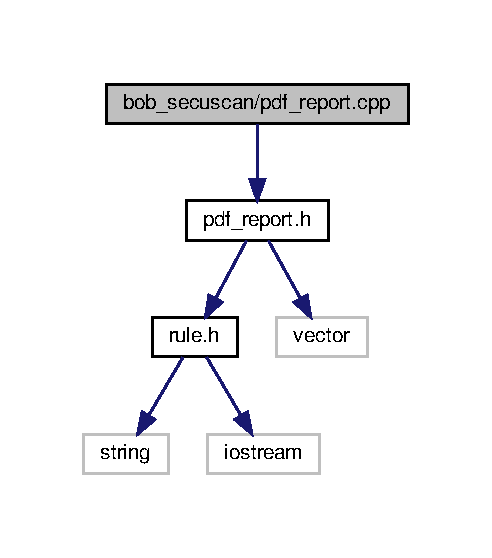
\includegraphics[width=236pt]{pdf__report_8cpp__incl}
\end{center}
\end{figure}
\subsection*{함수}
\begin{DoxyCompactItemize}
\item 
void \hyperlink{pdf__report_8cpp_a9a68b1bf8ea084181a40a5296be9d805}{create\+\_\+pdf} (vector$<$ \hyperlink{struct_rule}{Rule} $>$ \&ruleset, int $\ast$pf)
\end{DoxyCompactItemize}


\subsection{함수 문서화}
\mbox{\Hypertarget{pdf__report_8cpp_a9a68b1bf8ea084181a40a5296be9d805}\label{pdf__report_8cpp_a9a68b1bf8ea084181a40a5296be9d805}} 
\index{pdf\+\_\+report.\+cpp@{pdf\+\_\+report.\+cpp}!create\+\_\+pdf@{create\+\_\+pdf}}
\index{create\+\_\+pdf@{create\+\_\+pdf}!pdf\+\_\+report.\+cpp@{pdf\+\_\+report.\+cpp}}
\subsubsection{\texorpdfstring{create\+\_\+pdf()}{create\_pdf()}}
{\footnotesize\ttfamily void create\+\_\+pdf (\begin{DoxyParamCaption}\item[{vector$<$ \hyperlink{struct_rule}{Rule} $>$ \&}]{ruleset,  }\item[{int $\ast$}]{pf }\end{DoxyParamCaption})}

html report 생성 

pdf\+\_\+report.\+cpp 파일의 3 번째 라인에서 정의되었습니다.


\begin{DoxyCode}
3                                                \{
4 
5 \}
\end{DoxyCode}
이 함수를 호출하는 함수들에 대한 그래프입니다.\+:\nopagebreak
\begin{figure}[H]
\begin{center}
\leavevmode
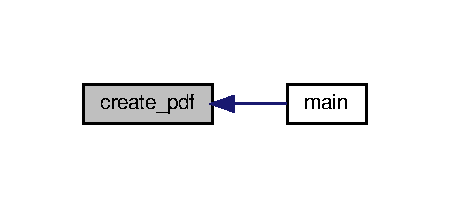
\includegraphics[width=216pt]{pdf__report_8cpp_a9a68b1bf8ea084181a40a5296be9d805_icgraph}
\end{center}
\end{figure}

\hypertarget{pdf__report_8h}{}\section{bob\+\_\+secuscan/pdf\+\_\+report.h 파일 참조}
\label{pdf__report_8h}\index{bob\+\_\+secuscan/pdf\+\_\+report.\+h@{bob\+\_\+secuscan/pdf\+\_\+report.\+h}}
{\ttfamily \#include \char`\"{}rule.\+h\char`\"{}}\newline
{\ttfamily \#include $<$vector$>$}\newline
pdf\+\_\+report.\+h에 대한 include 의존 그래프\nopagebreak
\begin{figure}[H]
\begin{center}
\leavevmode
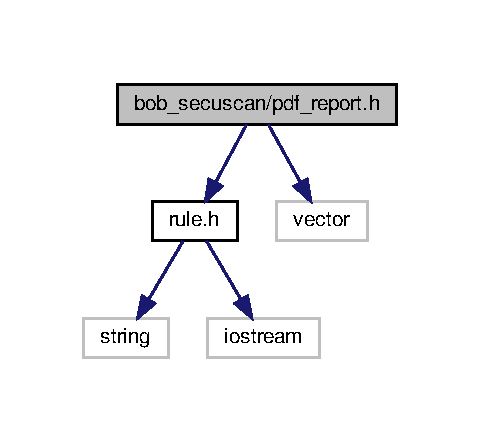
\includegraphics[width=231pt]{pdf__report_8h__incl}
\end{center}
\end{figure}
이 그래프는 이 파일을 직/간접적으로 include 하는 파일들을 보여줍니다.\+:\nopagebreak
\begin{figure}[H]
\begin{center}
\leavevmode
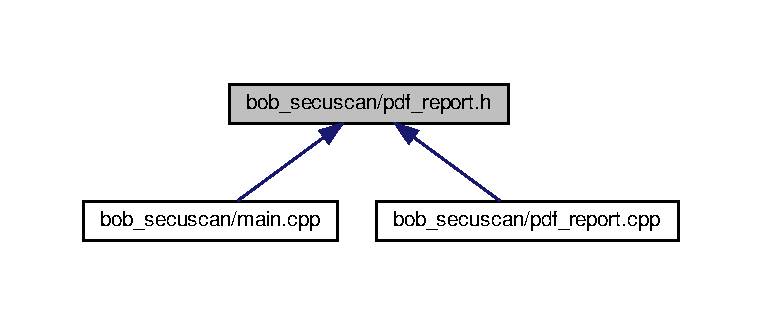
\includegraphics[width=350pt]{pdf__report_8h__dep__incl}
\end{center}
\end{figure}
\subsection*{함수}
\begin{DoxyCompactItemize}
\item 
void \hyperlink{pdf__report_8h_a9a68b1bf8ea084181a40a5296be9d805}{create\+\_\+pdf} (vector$<$ \hyperlink{struct_rule}{Rule} $>$ \&ruleset, int $\ast$pf)
\end{DoxyCompactItemize}


\subsection{함수 문서화}
\mbox{\Hypertarget{pdf__report_8h_a9a68b1bf8ea084181a40a5296be9d805}\label{pdf__report_8h_a9a68b1bf8ea084181a40a5296be9d805}} 
\index{pdf\+\_\+report.\+h@{pdf\+\_\+report.\+h}!create\+\_\+pdf@{create\+\_\+pdf}}
\index{create\+\_\+pdf@{create\+\_\+pdf}!pdf\+\_\+report.\+h@{pdf\+\_\+report.\+h}}
\subsubsection{\texorpdfstring{create\+\_\+pdf()}{create\_pdf()}}
{\footnotesize\ttfamily void create\+\_\+pdf (\begin{DoxyParamCaption}\item[{vector$<$ \hyperlink{struct_rule}{Rule} $>$ \&}]{ruleset,  }\item[{int $\ast$}]{pf }\end{DoxyParamCaption})}

html report 생성 

pdf\+\_\+report.\+cpp 파일의 3 번째 라인에서 정의되었습니다.


\begin{DoxyCode}
3                                                \{
4 
5 \}
\end{DoxyCode}
이 함수를 호출하는 함수들에 대한 그래프입니다.\+:\nopagebreak
\begin{figure}[H]
\begin{center}
\leavevmode
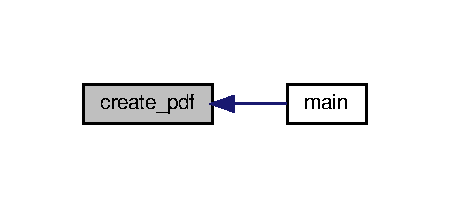
\includegraphics[width=216pt]{pdf__report_8h_a9a68b1bf8ea084181a40a5296be9d805_icgraph}
\end{center}
\end{figure}

\hypertarget{rule_8cpp}{}\section{bob\+\_\+secuscan/rule.cpp 파일 참조}
\label{rule_8cpp}\index{bob\+\_\+secuscan/rule.\+cpp@{bob\+\_\+secuscan/rule.\+cpp}}
{\ttfamily \#include \char`\"{}rule.\+h\char`\"{}}\newline
rule.\+cpp에 대한 include 의존 그래프\nopagebreak
\begin{figure}[H]
\begin{center}
\leavevmode
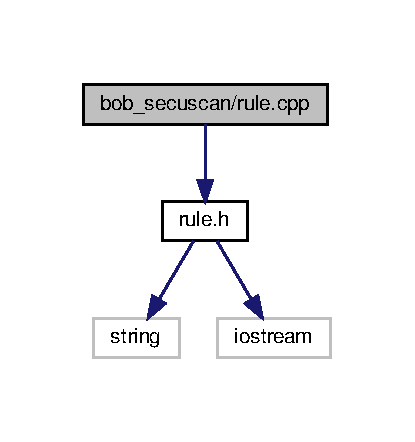
\includegraphics[width=199pt]{rule_8cpp__incl}
\end{center}
\end{figure}

\hypertarget{rule_8h}{}\section{bob\+\_\+secuscan/rule.h 파일 참조}
\label{rule_8h}\index{bob\+\_\+secuscan/rule.\+h@{bob\+\_\+secuscan/rule.\+h}}
{\ttfamily \#include $<$string$>$}\newline
{\ttfamily \#include $<$iostream$>$}\newline
rule.\+h에 대한 include 의존 그래프
\nopagebreak
\begin{figure}[H]
\begin{center}
\leavevmode
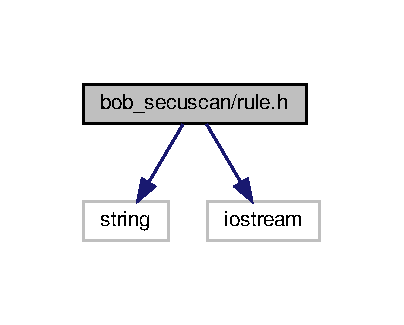
\includegraphics[width=194pt]{rule_8h__incl}
\end{center}
\end{figure}
이 그래프는 이 파일을 직/간접적으로 include 하는 파일들을 보여줍니다.\+:
\nopagebreak
\begin{figure}[H]
\begin{center}
\leavevmode
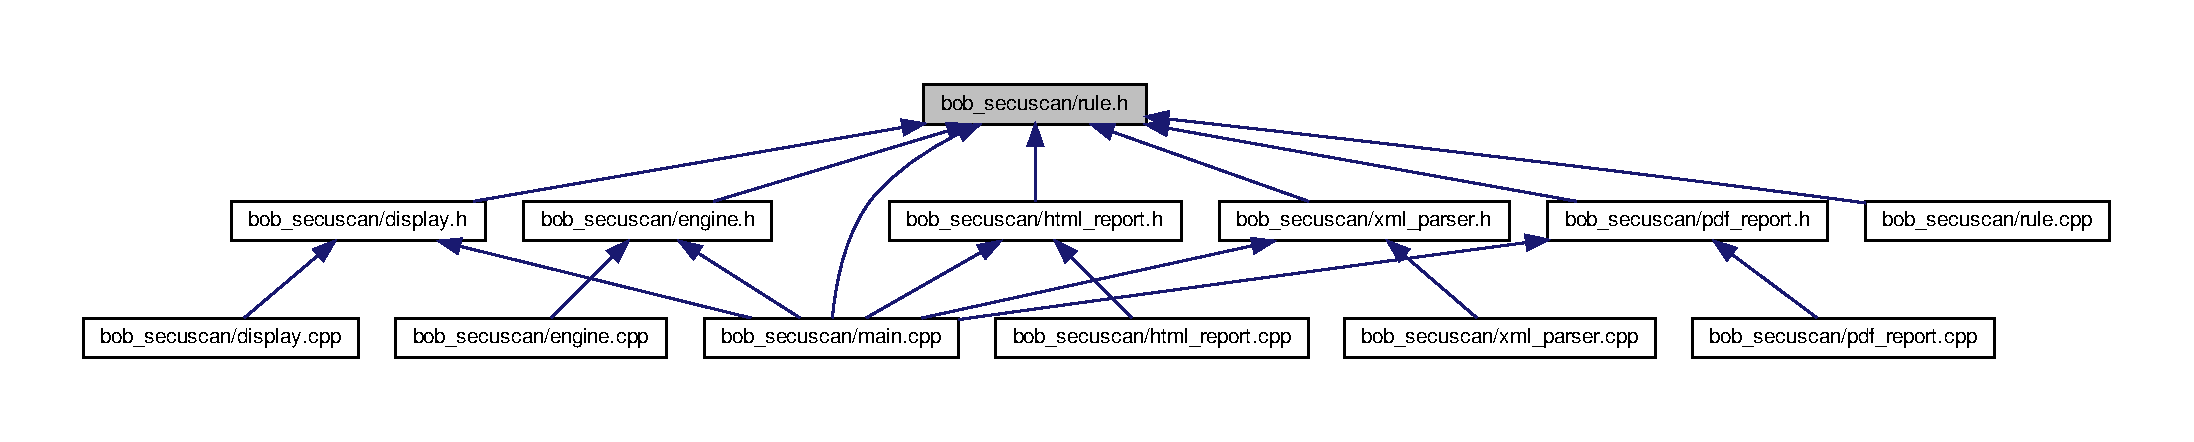
\includegraphics[width=350pt]{rule_8h__dep__incl}
\end{center}
\end{figure}
\subsection*{클래스}
\begin{DoxyCompactItemize}
\item 
struct \hyperlink{struct_rule}{Rule}
\end{DoxyCompactItemize}

\hypertarget{scoring_8cpp}{}\section{bob\+\_\+secuscan/scoring.cpp 파일 참조}
\label{scoring_8cpp}\index{bob\+\_\+secuscan/scoring.\+cpp@{bob\+\_\+secuscan/scoring.\+cpp}}
{\ttfamily \#include \char`\"{}scoring.\+h\char`\"{}}\newline
scoring.\+cpp에 대한 include 의존 그래프
\nopagebreak
\begin{figure}[H]
\begin{center}
\leavevmode
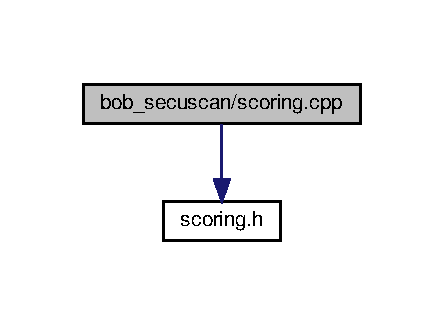
\includegraphics[width=213pt]{scoring_8cpp__incl}
\end{center}
\end{figure}
\subsection*{함수}
\begin{DoxyCompactItemize}
\item 
int \hyperlink{scoring_8cpp_afc65323578d43d64369eeeb29a163376}{cvss\+\_\+score} (int $\ast$passfail)
\end{DoxyCompactItemize}


\subsection{함수 문서화}
\mbox{\Hypertarget{scoring_8cpp_afc65323578d43d64369eeeb29a163376}\label{scoring_8cpp_afc65323578d43d64369eeeb29a163376}} 
\index{scoring.\+cpp@{scoring.\+cpp}!cvss\+\_\+score@{cvss\+\_\+score}}
\index{cvss\+\_\+score@{cvss\+\_\+score}!scoring.\+cpp@{scoring.\+cpp}}
\subsubsection{\texorpdfstring{cvss\+\_\+score()}{cvss\_score()}}
{\footnotesize\ttfamily int cvss\+\_\+score (\begin{DoxyParamCaption}\item[{int $\ast$}]{passfail }\end{DoxyParamCaption})}

cvss기준으로 점수 평가 

scoring.\+cpp 파일의 3 번째 라인에서 정의되었습니다.


\begin{DoxyCode}
3                              \{
4     \textcolor{keywordtype}{int} score=0;
5     \textcolor{keywordflow}{for}(\textcolor{keywordtype}{int} i=0; i<len(passfail); i++)\{
6         score+=cvss(passfail[i]);
7     \}
8 \}
\end{DoxyCode}
이 함수를 호출하는 함수들에 대한 그래프입니다.\+:
\nopagebreak
\begin{figure}[H]
\begin{center}
\leavevmode
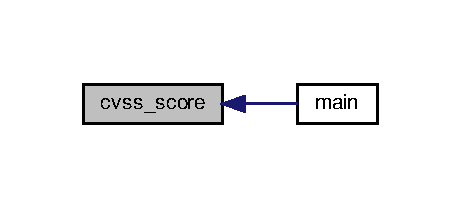
\includegraphics[width=221pt]{scoring_8cpp_afc65323578d43d64369eeeb29a163376_icgraph}
\end{center}
\end{figure}

\hypertarget{scoring_8h}{}\section{bob\+\_\+secuscan/scoring.h 파일 참조}
\label{scoring_8h}\index{bob\+\_\+secuscan/scoring.\+h@{bob\+\_\+secuscan/scoring.\+h}}
이 그래프는 이 파일을 직/간접적으로 include 하는 파일들을 보여줍니다.\+:\nopagebreak
\begin{figure}[H]
\begin{center}
\leavevmode
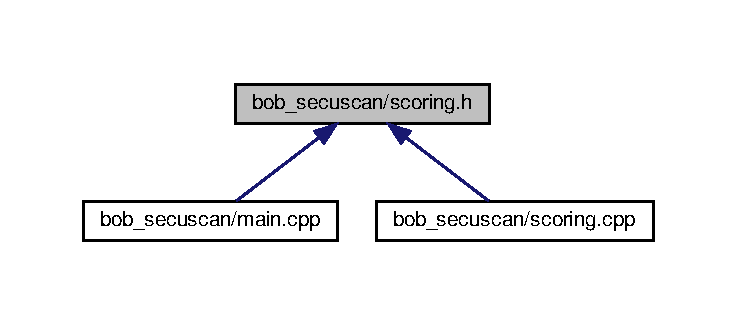
\includegraphics[width=350pt]{scoring_8h__dep__incl}
\end{center}
\end{figure}
\subsection*{함수}
\begin{DoxyCompactItemize}
\item 
int \hyperlink{scoring_8h_afc65323578d43d64369eeeb29a163376}{cvss\+\_\+score} (int $\ast$passfail)
\end{DoxyCompactItemize}


\subsection{함수 문서화}
\mbox{\Hypertarget{scoring_8h_afc65323578d43d64369eeeb29a163376}\label{scoring_8h_afc65323578d43d64369eeeb29a163376}} 
\index{scoring.\+h@{scoring.\+h}!cvss\+\_\+score@{cvss\+\_\+score}}
\index{cvss\+\_\+score@{cvss\+\_\+score}!scoring.\+h@{scoring.\+h}}
\subsubsection{\texorpdfstring{cvss\+\_\+score()}{cvss\_score()}}
{\footnotesize\ttfamily int cvss\+\_\+score (\begin{DoxyParamCaption}\item[{int $\ast$}]{passfail }\end{DoxyParamCaption})}

cvss기준으로 점수 평가 

scoring.\+cpp 파일의 3 번째 라인에서 정의되었습니다.


\begin{DoxyCode}
3                              \{
4     \textcolor{keywordtype}{int} score=0;
5     \textcolor{keywordflow}{for}(\textcolor{keywordtype}{int} i=0; i<len(passfail); i++)\{
6         score+=cvss(passfail[i]);
7     \}
8 \}
\end{DoxyCode}
이 함수를 호출하는 함수들에 대한 그래프입니다.\+:\nopagebreak
\begin{figure}[H]
\begin{center}
\leavevmode
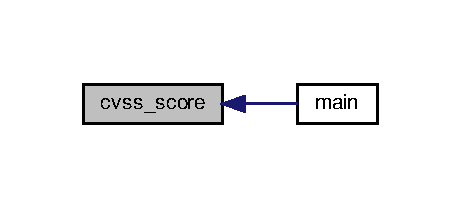
\includegraphics[width=221pt]{scoring_8h_afc65323578d43d64369eeeb29a163376_icgraph}
\end{center}
\end{figure}

\hypertarget{xml__parser_8cpp}{}\section{bob\+\_\+secuscan/xml\+\_\+parser.cpp 파일 참조}
\label{xml__parser_8cpp}\index{bob\+\_\+secuscan/xml\+\_\+parser.\+cpp@{bob\+\_\+secuscan/xml\+\_\+parser.\+cpp}}
{\ttfamily \#include \char`\"{}xml\+\_\+parser.\+h\char`\"{}}\newline
xml\+\_\+parser.\+cpp에 대한 include 의존 그래프
\nopagebreak
\begin{figure}[H]
\begin{center}
\leavevmode
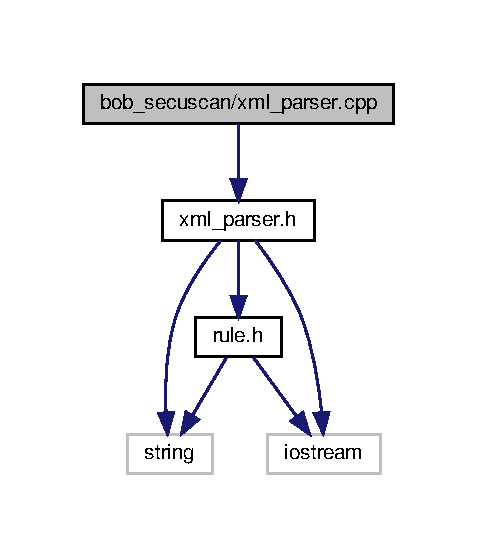
\includegraphics[width=229pt]{xml__parser_8cpp__incl}
\end{center}
\end{figure}
\subsection*{함수}
\begin{DoxyCompactItemize}
\item 
\hyperlink{struct_rule}{Rule} \hyperlink{xml__parser_8cpp_ad140c00557c11c4c2c8da2696684f9ea}{parse} (char $\ast$xml\+\_\+line)
\end{DoxyCompactItemize}


\subsection{함수 문서화}
\mbox{\Hypertarget{xml__parser_8cpp_ad140c00557c11c4c2c8da2696684f9ea}\label{xml__parser_8cpp_ad140c00557c11c4c2c8da2696684f9ea}} 
\index{xml\+\_\+parser.\+cpp@{xml\+\_\+parser.\+cpp}!parse@{parse}}
\index{parse@{parse}!xml\+\_\+parser.\+cpp@{xml\+\_\+parser.\+cpp}}
\subsubsection{\texorpdfstring{parse()}{parse()}}
{\footnotesize\ttfamily \hyperlink{struct_rule}{Rule} parse (\begin{DoxyParamCaption}\item[{char $\ast$}]{xml\+\_\+line }\end{DoxyParamCaption})}

parsing xml line by line 

xml\+\_\+parser.\+cpp 파일의 3 번째 라인에서 정의되었습니다.


\begin{DoxyCode}
3                           \{
4     \textcolor{keywordtype}{string} split\_xml[4];
5     split\_xml=split(xml\_line);
6     \textcolor{keywordtype}{string} definition=split\_xml[0];
7     \textcolor{keywordtype}{string} test=split\_xml[1];
8     \textcolor{keywordtype}{string} \textcolor{keywordtype}{object}=split\_xml[2];
9     \textcolor{keywordtype}{string} state=split\_xml[3];
10     \textcolor{keywordtype}{string} \hyperlink{engine_8cpp_a0f15a8265e6f3a4a16da1286c6659721}{fixation}=split\_xml[4];
11     \hyperlink{struct_rule}{Rule} newrule=\hyperlink{struct_rule}{Rule}(definition, test, \textcolor{keywordtype}{object}, state, fixation);
12     \textcolor{keywordflow}{return} newrule;
13 \}
\end{DoxyCode}
이 함수 내부에서 호출하는 함수들에 대한 그래프입니다.\+:
\nopagebreak
\begin{figure}[H]
\begin{center}
\leavevmode
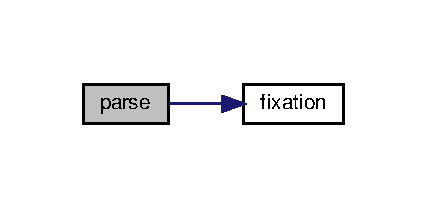
\includegraphics[width=205pt]{xml__parser_8cpp_ad140c00557c11c4c2c8da2696684f9ea_cgraph}
\end{center}
\end{figure}

\hypertarget{xml__parser_8h}{}\section{bob\+\_\+secuscan/xml\+\_\+parser.h 파일 참조}
\label{xml__parser_8h}\index{bob\+\_\+secuscan/xml\+\_\+parser.\+h@{bob\+\_\+secuscan/xml\+\_\+parser.\+h}}
{\ttfamily \#include \char`\"{}rule.\+h\char`\"{}}\newline
{\ttfamily \#include $<$string$>$}\newline
{\ttfamily \#include $<$iostream$>$}\newline
xml\+\_\+parser.\+h에 대한 include 의존 그래프
\nopagebreak
\begin{figure}[H]
\begin{center}
\leavevmode
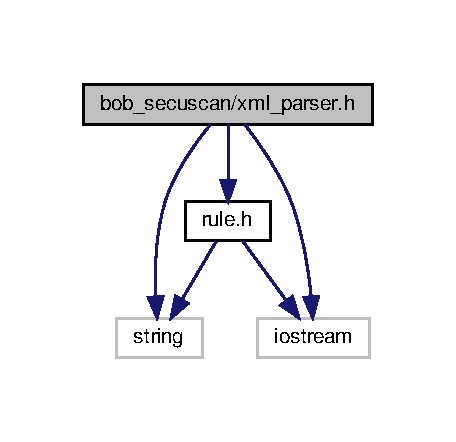
\includegraphics[width=219pt]{xml__parser_8h__incl}
\end{center}
\end{figure}
이 그래프는 이 파일을 직/간접적으로 include 하는 파일들을 보여줍니다.\+:
\nopagebreak
\begin{figure}[H]
\begin{center}
\leavevmode
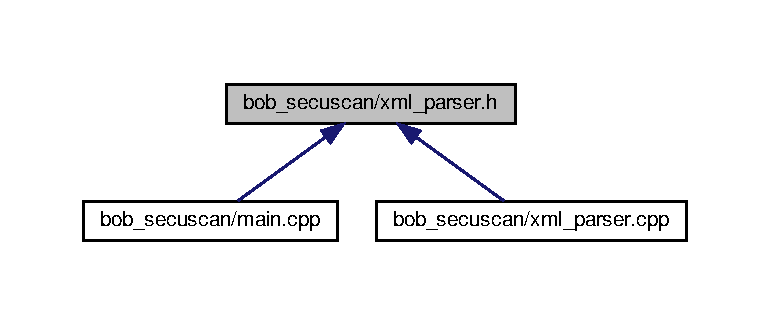
\includegraphics[width=350pt]{xml__parser_8h__dep__incl}
\end{center}
\end{figure}
\subsection*{함수}
\begin{DoxyCompactItemize}
\item 
\hyperlink{struct_rule}{Rule} \hyperlink{xml__parser_8h_ad140c00557c11c4c2c8da2696684f9ea}{parse} (char $\ast$xml\+\_\+line)
\end{DoxyCompactItemize}


\subsection{함수 문서화}
\mbox{\Hypertarget{xml__parser_8h_ad140c00557c11c4c2c8da2696684f9ea}\label{xml__parser_8h_ad140c00557c11c4c2c8da2696684f9ea}} 
\index{xml\+\_\+parser.\+h@{xml\+\_\+parser.\+h}!parse@{parse}}
\index{parse@{parse}!xml\+\_\+parser.\+h@{xml\+\_\+parser.\+h}}
\subsubsection{\texorpdfstring{parse()}{parse()}}
{\footnotesize\ttfamily \hyperlink{struct_rule}{Rule} parse (\begin{DoxyParamCaption}\item[{char $\ast$}]{xml\+\_\+line }\end{DoxyParamCaption})}

parsing xml line by line 

xml\+\_\+parser.\+cpp 파일의 3 번째 라인에서 정의되었습니다.


\begin{DoxyCode}
3                           \{
4     \textcolor{keywordtype}{string} split\_xml[4];
5     split\_xml=split(xml\_line);
6     \textcolor{keywordtype}{string} definition=split\_xml[0];
7     \textcolor{keywordtype}{string} test=split\_xml[1];
8     \textcolor{keywordtype}{string} \textcolor{keywordtype}{object}=split\_xml[2];
9     \textcolor{keywordtype}{string} state=split\_xml[3];
10     \textcolor{keywordtype}{string} \hyperlink{engine_8cpp_a0f15a8265e6f3a4a16da1286c6659721}{fixation}=split\_xml[4];
11     \hyperlink{struct_rule}{Rule} newrule=\hyperlink{struct_rule}{Rule}(definition, test, \textcolor{keywordtype}{object}, state, fixation);
12     \textcolor{keywordflow}{return} newrule;
13 \}
\end{DoxyCode}
이 함수 내부에서 호출하는 함수들에 대한 그래프입니다.\+:
\nopagebreak
\begin{figure}[H]
\begin{center}
\leavevmode
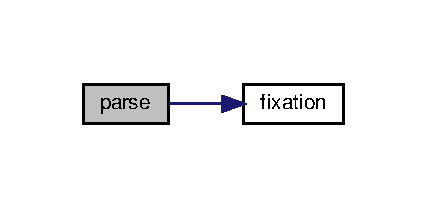
\includegraphics[width=205pt]{xml__parser_8h_ad140c00557c11c4c2c8da2696684f9ea_cgraph}
\end{center}
\end{figure}

%--- End generated contents ---

% Index
\backmatter
\newpage
\phantomsection
\clearemptydoublepage
\addcontentsline{toc}{chapter}{색인}
\printindex

\end{document}
